\chapter{Evolution of heterogeneous ensembles through dynamic particle swarm optimization for video-based face recognition}

After performing mono-optimization of only one FAM network when new data is available, this chapter presents a second iteration of the supervised incremental learning strategy that optimizes a population of classifiers to create ensembles.
Whereas the previous study illustrates the impact of learning new data incrementally on the optimization environment, this chapter focuses on characterizing how genotype (\emph{i.e.}, hyperparameter) diversity affects classifier diversity and how this relationship can be used to evolve diversified ensembles of classifiers.
It was published in the Pattern Recognition journal (Elsevier) \cite{connolly11}. 

%----------------------------- Abstract & keywords ----------------------------%
%-- Paper objective
In this chapter, an incremental learning strategy based on dynamic particle swarm optimization (DPSO) is proposed to evolve heterogeneous ensembles of classifiers (where each classifier corresponds to a particle) in response to new reference samples.
This new strategy is applied to video-based face recognition, using an adaptive multiclassifier system (AMCS) that consists of a pool of fuzzy ARTMAP (FAM) neural networks for classification of facial regions, and a niching version of DPSO that optimizes all FAM parameters such that the classification rate is maximized.
%-- Results
Given that diversity within a dynamic particle swarm is correlated with diversity within a corresponding pool of base classifiers, DPSO properties are exploited to generate and evolve diversified pools of FAM classifiers, and to efficiently select ensembles among the pools based on accuracy and particle swarm diversity.
Performance of the proposed strategy is assessed in terms of classification rate and resource requirements under different incremental learning scenarios, where new reference data is extracted from real-world video streams.
%-- Results presentation - generality
Simulation results indicate the DPSO strategy provides an efficient way to evolve ensembles of FAM networks in an AMCS.
Maintaining particle diversity in the optimization space yields a level of accuracy that is comparable to AMCS using reference ensemble-based and batch learning techniques, but requires significantly lower computational complexity than assessing diversity among classifiers in the feature or decision spaces.

%------------------------------------ Text ------------------------------------%
\section{Introduction}

In pattern recognition systems, neural or statistical classifiers define class models (or hypotheses), using data samples defined in a $\mathbb{R}^I$ input feature space (also referred to as hypothesis space in \cite{brown05}), and map those models to a decision space to perform predictions.
Exploiting several views of a same problem with classifier ensembles has been shown to improve the overall accuracy and reliability for a wide range of applications.
However, generating an accurate pool of base classifiers and selecting an ensemble among that pool that maximizes prediction precision are challenging tasks.
One key element in the success of classifiers ensembles that has attracted a great deal of interest in recent years is \emph{classifier diversity measures} (\cite{canuto07, hadjitodorov06, kapp07, oliveira09, sirlantzis08, ulas09}).
Since diversity is difficult to assess in the input feature space, these measures compute the disagreement between classifiers in the decision space, over several predictions.
Through bias-variance error decomposition, it has been shown empirically that considering diversity for ensemble selection improves the generalization capabilities of multiple classifiers systems (\cite{brown05}).

%-------------------------------- Environments --------------------------------%
\begin{figure*}[tb]
  \centering
  \fbox{
  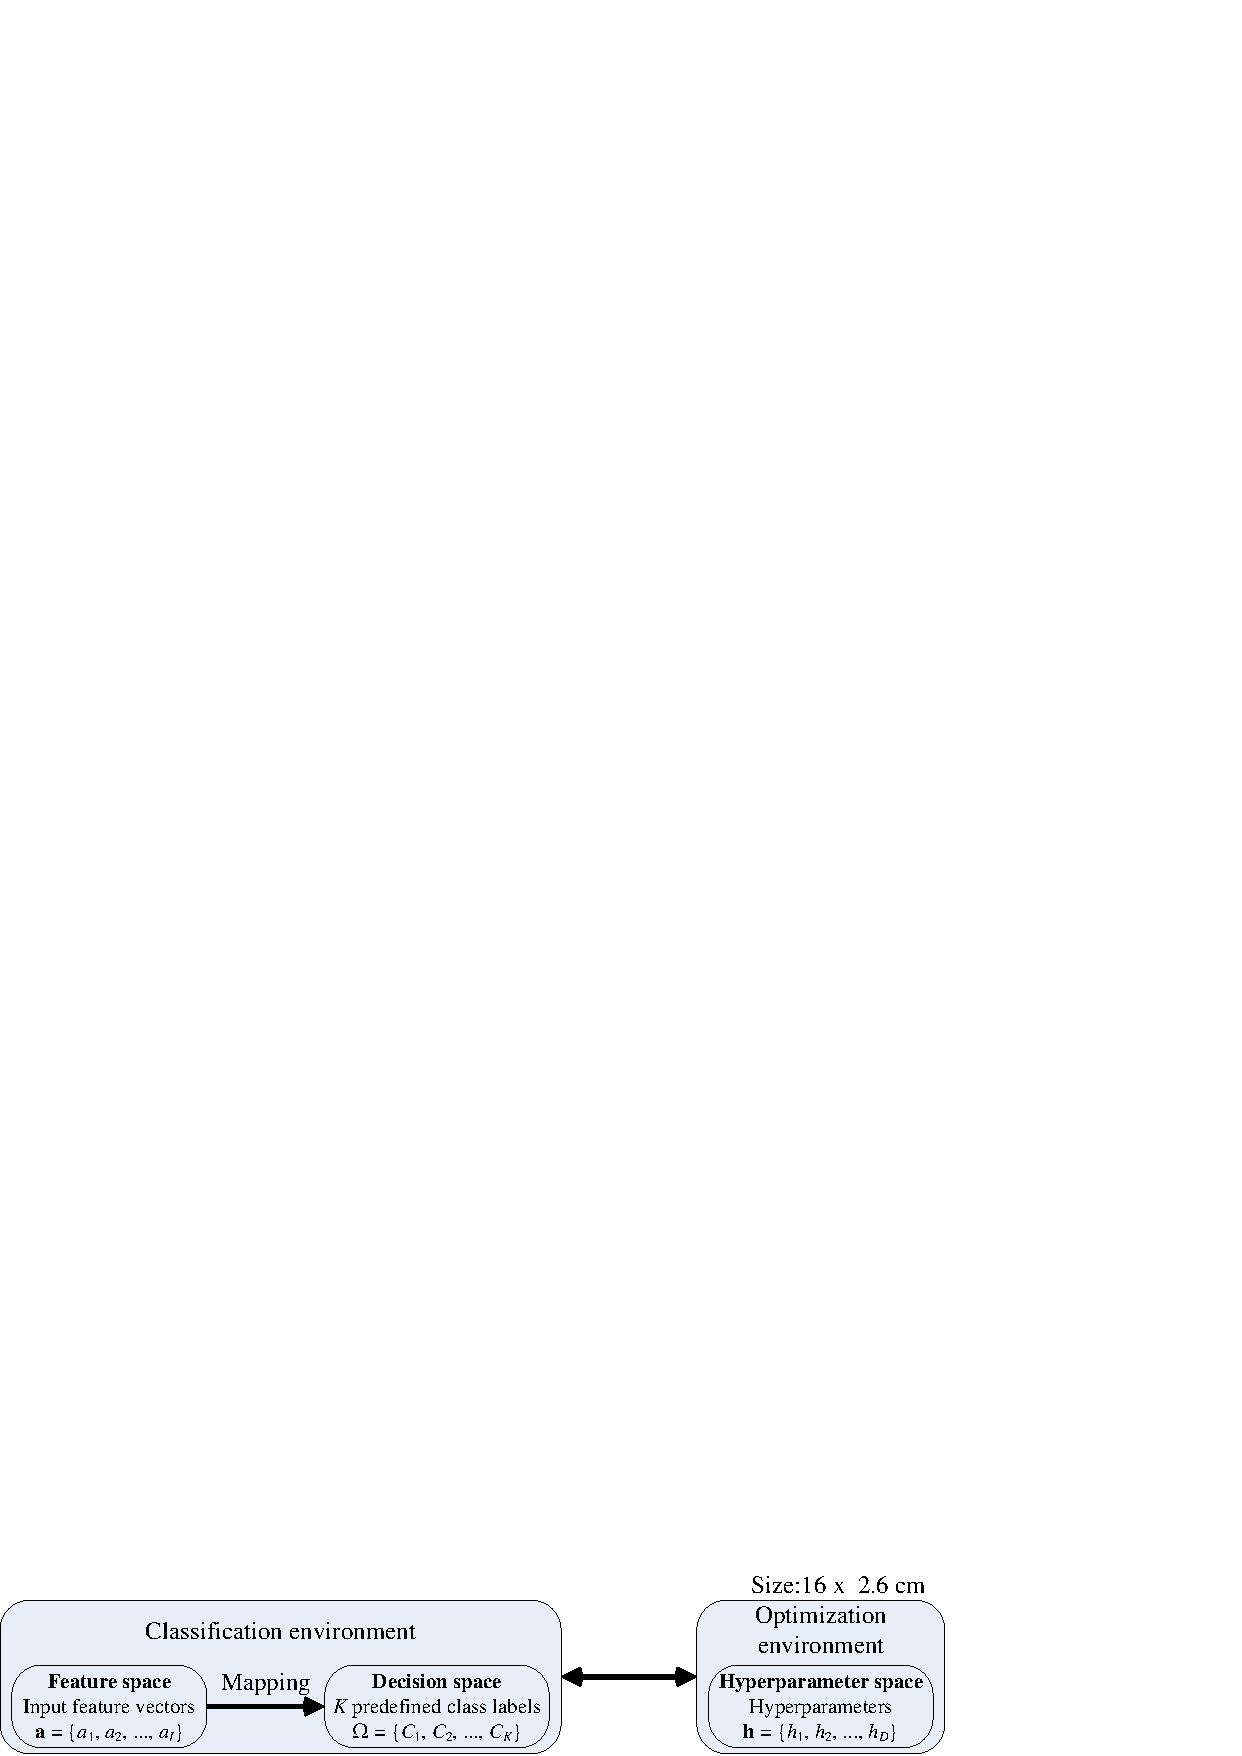
\includegraphics[width=0.9\linewidth, viewport=0cm 0cm 16.01cm 2.64cm, clip]
                  {c2_fig1}  }
  \caption{Pattern classification systems may be defined according to two environments.
A \emph{classification environment} that maps a $\mathbb{R}^I$ input feature space to a decision space, respectively defined by feature vectors \textbf{a}, and a set of class labels $\Omega$.
Interacting with the latter is an \emph{optimization environment}, where each vector \textbf{h} indicates a position in the hyperparameter space defined according a classifier's learning algorithm.
The representation space traversal seeks to maintaining diversity among classifiers by exploiting the interaction between these two environments.
The basic assumption is that different positions in the hyperparameter space lead to different class models in the feature space, and thus different class label $C_k$ predictions in the decision space}
	\label{fig:c2_environments}
\end{figure*}
%------------------------------- \Environments --------------------------------%

Diversity can be achieved via (1) different starting points in the input feature space, using a learning algorithm trained with different initial conditions, (2) different sets of accessible hypotheses using different training data sets (\emph{e.g.}, boosting and bagging) or different learning algorithms, and (3) representation space traversal that optimizes parameters, using a penalty term or evolutionary method, to ensure that base classifiers occupy different areas in the feature space.
In the latter case, the hyperparameters of a classifier (\emph{e.g.}, learning rate) define an optimization space (\cite{granger07}).
As described in Figure \ref{fig:c2_environments}, supervised learning strategies may then allow to optimize a classifier's hyperparameters such as accuracy is maximized.
Since these hyperparameters govern the learning dynamics of a classifier, diversity among solutions in the \emph{optimization environment} leads to ensemble diversity in the \emph{classification environment}.
Diversity can thus be maintained without relying on costly classifier diversity measures.

%-- Biometric / face recognition
The recognition of individuals based on their biometric traits provides a powerful alternative to traditional authentication schemes that are presently applied in security and surveillance systems.
In biometric applications, such as face recognition in video, the collection and analysis of labeled reference samples to design biometric systems (during an enrollment of re-enrollment process) is often expensive and time consuming.
Samples acquired from video streams in \emph{unconstrained} scenes are generally of poor quality with low resolution, resulting in classifiers applied to biometric matching that are often trained with limited and unbalanced data with much inter- and intra-class variability, 
Moreover, given that facial regions are often captured discreetly, without cooperation, they are subject to considerable variations due to limited control over operational conditions (\emph{e.g.}, illumination, pose, facial expression, orientation and occlusion).
In addition, operating conditions and individual physiology may even change over time, either temporary (\emph{e.g.}, haircut, glasses, lighting, etc.) or permanently (\emph{e.g.}, scars, aging).
New informations, such as input features and output classes, may suddenly emerge and previously acquired data may eventually become obsolete in dynamically changing classification environments (\cite{granger01, tsymbal08}).
These factors contribute to a growing divergence between the biometric model of an individual and its underlying class distribution.\footnote{Typically designed during an a priori enrollment phase, the biometric model of an individual for matching consists of one or more templates (reference samples) or the parameters statistical or structural model of reference samples.}

It is common in many biometric applications to acquire additional data and knowledge from the environment or other sources over time, after the system has originally been deployed for operations.
For accurate recognition of individuals, biometric systems should adapt their models over time in response to new or changing input features, data samples, priors, classes and environments.
In this chapter, it is assumed that new reference data becomes available to create new biometric models when individuals enroll to the system, and to update models of individuals previously enrolled to the system. 
Some adaptive biometric systems have been proposed in the literature to refine biometric models according to the intra-class variations in input samples (\cite{roli08}).
Indeed, with self-adaptive or semi-supervised learning strategies, biometric models are initially designed during enrollment using labeled training data, and then updated with highly confident unlabeled data obtained during operations (\cite{poh09, rattani10}).
These strategies are however vulnerable to outliers, dispersion and overlap in class distributions.
Stringent criteria are required for selection of highly confident data, to minimize the probability of introducing impostor data into updated biometric models.
In this chapter, supervised learning strategies are considered, and new data samples are assumed to be analyzed and labeled by an operator with expert knowledge of intra-class variations.
Labeled data becomes available, for instance, over multiple (re)enrollment sessions, or when operational scenarios are analyzed off-line, and can allow an operator to gradually build the biometric models of a system over time.
Adaptive biometric systems in literature have used newly-acquired reference samples to update the selection of a user's template from a gallery via clustering and editing techniques (\cite{uludag04}).
Others have performed on-line learning of genuine samples over time to update each user's single super template (\cite{jiang02}).
It is however difficult to represent intra-class variations with a single template (\cite{roli08}).

In previous work, the authors proposed an adaptive classification system (ACS) to update biometric models of individuals in response to new labeled reference data from the operational environment during video-based face recognition (\cite{connolly10}).
It uses the fuzzy ARTMAP (FAM) neural network for supervised incremental learning of limited data, as well as fast and efficient matching of facial regions detected in video streams against the model of individuals enrolled to a face recognition system.
The authors have showed that (1) adaptation of a FAM network during supervised incremental learning is a dynamic optimization problem in the hyperparameter space, and (2) corruption of the biometric models resulting from incremental learning of new data can be reduced using an ensemble-based approach (\cite{connolly10_2}).
It exist several directions to address uncertain classification environments with ensembles, such as changing classifier combination rules, updating classifiers using the new reference data, and changing ensemble structure by replacing old or underperforming members (\cite{kuncheva04}).
However, few of these approaches explicitly exploit classifier diversity when adapting ensembles over time in a context where to few data are available.

Given the limited amount of data available to design biometric systems, creating diversity among classifiers through \emph{representation space traversal} is an efficient way to exploit those data to provide reliable classifier ensembles.
For instance, with a cooperative neural network co-evolution paradigm (\cite{potter00}), evolutionary algorithms have been used to create \emph{heterogeneous} ensembles (\cite{valentini03}).\footnote{This definition differs with respect to certain other definitions of heterogeneous ensembles found in literature (\cite{oliveira09, rashid09}).}
It allows, exploring a hyperparameter space to train classifiers of the same type, on the same data, but with different learning dynamics.
These approaches, where classifiers cooperate, exchange information, but yet have their design and training be independent, have been shown to provide more accurate ensembles (\cite{bakker03, garcia05, liu01, zhou02}).

%-- Objective
In this chapter, the relationship between diversity in the classification and optimization environments is exploited for efficient design of heterogeneous ensembles of classifiers in video-based face recognition. 
Under the hypothesis that diversity in the hyperparameter space is correlated with diversity among a corresponding pool of classifiers in the feature and decision spaces, a specialized learning strategy based on dynamic particle swarm optimization (DPSO) is proposed for supervised incremental learning of new data.
This incremental DPSO-based learning strategy is applied to an adaptive multiclassifier system (AMCS) that consists of a pool FAM networks (\cite{carpenter92}) for classification that interacts with a niching version of DPSO (\cite{nickabadi08_2}).
The DPSO-based learning strategy incrementally evolves a heterogeneous ensemble of FAM networks in response to new reference data.
Each particle in the optimization environment corresponds to a FAM network in the classification environment, and the DPSO strategy cojointly optimizes \emph{all classifier parameters} -- hyperparameters, weights, and architecture -- of a pool of classifiers such as classification rate is maximized.
The ability of DPSO algorithms to find and track several changing local optima in the hyperparameter space is exploited by the AMCS to create a diversified pool (or swarm) of \emph{heterogeneous} classifiers.
DPSO properties are applied in a novel greedy search process to efficiently select an ensemble among the pool of FAM classifiers, based on accuracy and particle swarm diversity.

This study focuses on video-based face recognition applications in which two incremental learning scenarios may occur--enrollment and update of facial models.
Performance of this system is assessed in terms of classification rate and resource requirements for incremental learning of new data blocks from two real-world video data sets--Institute of Information Technology of the Canadian National Research Council (IIT-NRC) (\cite{gorodnichy05}) and Motion of Body (MoBo) (\cite{gross02}).
In proof-of-concept experiments, the AMCS performs biometric matching of facial regions against the facial model of individuals enrolled to a system for closed-set identification.
Finally, the relationship between diversity in a classifier's hyperparameter space and diversity in it's feature and decision space is analyzed for both batch and incremental learning cases.

%-- Structure
In Section \ref{sec:c2_adaptation}, the AMCS is described along with the FAM network used for classification, and the DPSO algorithm used to optimize system parameters.
In Section \ref{sec:c2_algo}, the new DPSO-based incremental learning strategy used to evolve heterogeneous ensembles is described.
Application, data bases, incremental learning scenarios, protocol, and performance measures used for proof-of-concept simulations are described in Section \ref{sec:c2_methodology}.
Finally, experimental results are presented and discussed in Section \ref{sec:c2_results_discussion}.

%--------------------------------- Adaptation ---------------------------------%
\section{An adaptive multiclassifier system}
\label{sec:c2_adaptation}

%------------------------- Framework - for section 2 --------------------------%
\begin{figure*}[t]
  \centering
  \fbox{
  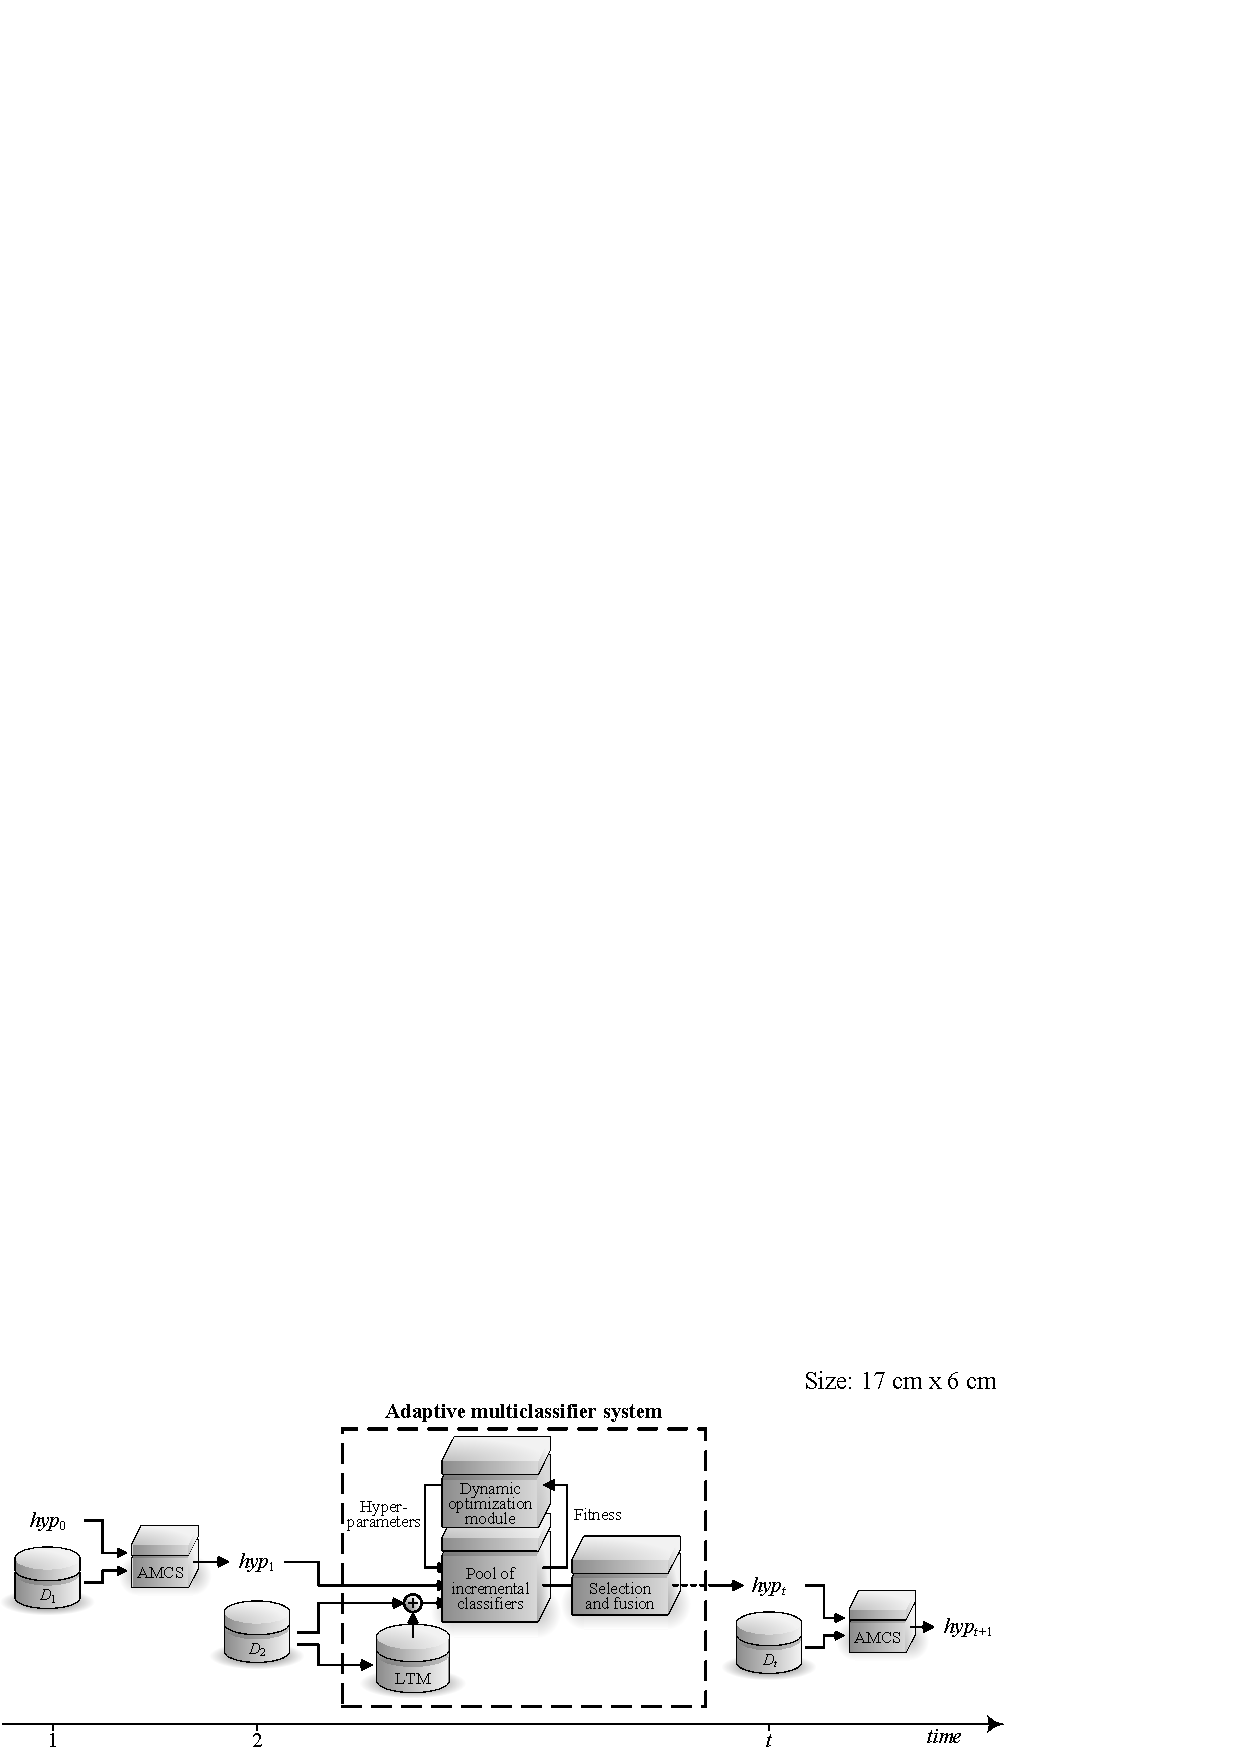
\includegraphics[width =0.97\linewidth, viewport =0cm 0cm 17cm 6cm, clip]
  								{c2_fig2} }
  \caption{Evolution over time of the adaptive multiclassifier system (AMCS) in a generic incremental learning scenario, where new blocks of data are used to update a swarm of classifiers.
Let $D_1$, $D_2$, ... be blocks of learning data that become available at different labeled instants in time $t=1,2,...,T$.
The AMCS starts with an initial hypothesis $hyp_0$ according to prior knowledge of the domain.
Each hypothesis $hyp_{t-1}$ are updated to $hyp_{t}$ by the AMCS on the basis of a new data blocks $D_t$}
	\label{fig:c2_framework}
\end{figure*}
%------------------------- \Framework - for section 2 -------------------------%

Figure \ref{fig:c2_framework} depicts the evolution of an adaptive multiclassifier system (AMCS) for supervised incremental learning of new reference labeled samples.
It is composed of a pool of base classifiers, each one suitable for supervised incremental learning, a dynamic evolutionary optimization module that tunes the user-defined hyperparameters of each classifier, and a long term memory (LTM) that stores and manages incoming data for validation.
This system differs from the system originally proposed in that a new DPSO incremental learning strategy allow to efficiently form a heterogeneous ensemble of classifiers (\cite{connolly10}).
It evolves a pool of classifiers, and is now composed of a selection and fusion module for efficient combination of heterogeneous ensembles.

When a new block of learning data $D_t$ becomes available to the system at a discrete time $t$, it is employed to update the LTM, and evolve the pool, or swarm, of incremental classifiers.
Each classifier is associated to a particle in the hyperparameter space, and a dynamic optimization module using a DPSO-based learning strategy cojointly determines the classifiers hyperparameters, architecture, and parameters such that classification rate is maximized (\cite{connolly10_2}).
Once the optimization process is complete, the selection and fusion module produces a heterogeneous ensemble by selecting and combining classifiers from the swarm, based on their accuracy and diversity.
The LTM stores data samples from each individual class for validation during incremental learning and fitness estimation of particles on the objective function (\cite{connolly10}).
The data from $D_t$ is partitioned and combined with that of the LTM to create three subsets: a training data set $D_t^\text{t}$, a validation data set $D_t^\text{v}$, and a fitness estimation data set $D_t^\text{f}$. 

In this chapter, a particular realization of this AMCS is considered.
The fuzzy ARTMAP (FAM) neural network (\cite{carpenter92}) is employed for incremental learning classification and a dynamical niching particle swarm optimization (DNPSO) algorithm (\cite{nickabadi08_2}) is used for dynamic optimization.
The rest of this section provides additional details on the FAM classifier and the DNPSO algorithm used within the AMCS.

%------------------------------------------------------------------------------%
%------------------------- Subsection : fuzzy ARTMAP --------------------------%
\subsection{Fuzzy ARTMAP neural network classifiers}
\label{sec:c2_fam}

Fuzzy ARTMAP (\cite{carpenter91}) is a versatile neural classifier that may provide a high level of prediction accuracy with moderate time and memory complexity (\cite{granger07}).
As such, fuzzy ARTMAP has been successfully applied to a wide variety of pattern recognition problems.
It is very promising for fast and efficient for biometric matching (of feature patterns against the model of individuals enrolled to a face recognition system) due to its ability to perform fast, stable, on-line, unsupervised or supervised, and incremental learning from limited amount of training data. 
A key feature of the ARTMAP networks is their unique solution to the stability-plasticity dilemma.
The popular fuzzy ARTMAP integrates the fuzzy ART to process both analog and binary-valued input patterns to the original ARTMAP architecture (\cite{carpenter92}).
Several other ARTMAP networks have been proposed to address this architecture to specific problems.
Members of the ARTMAP family can be broadly divided according to their internal matching process, which depends on either deterministic or probabilistic category activation (\cite{connolly09}).

%-------------------------------- Fuzzy ARTMAP --------------------------------%
\begin{figure*}[!t]
  \centering
  \fbox{
  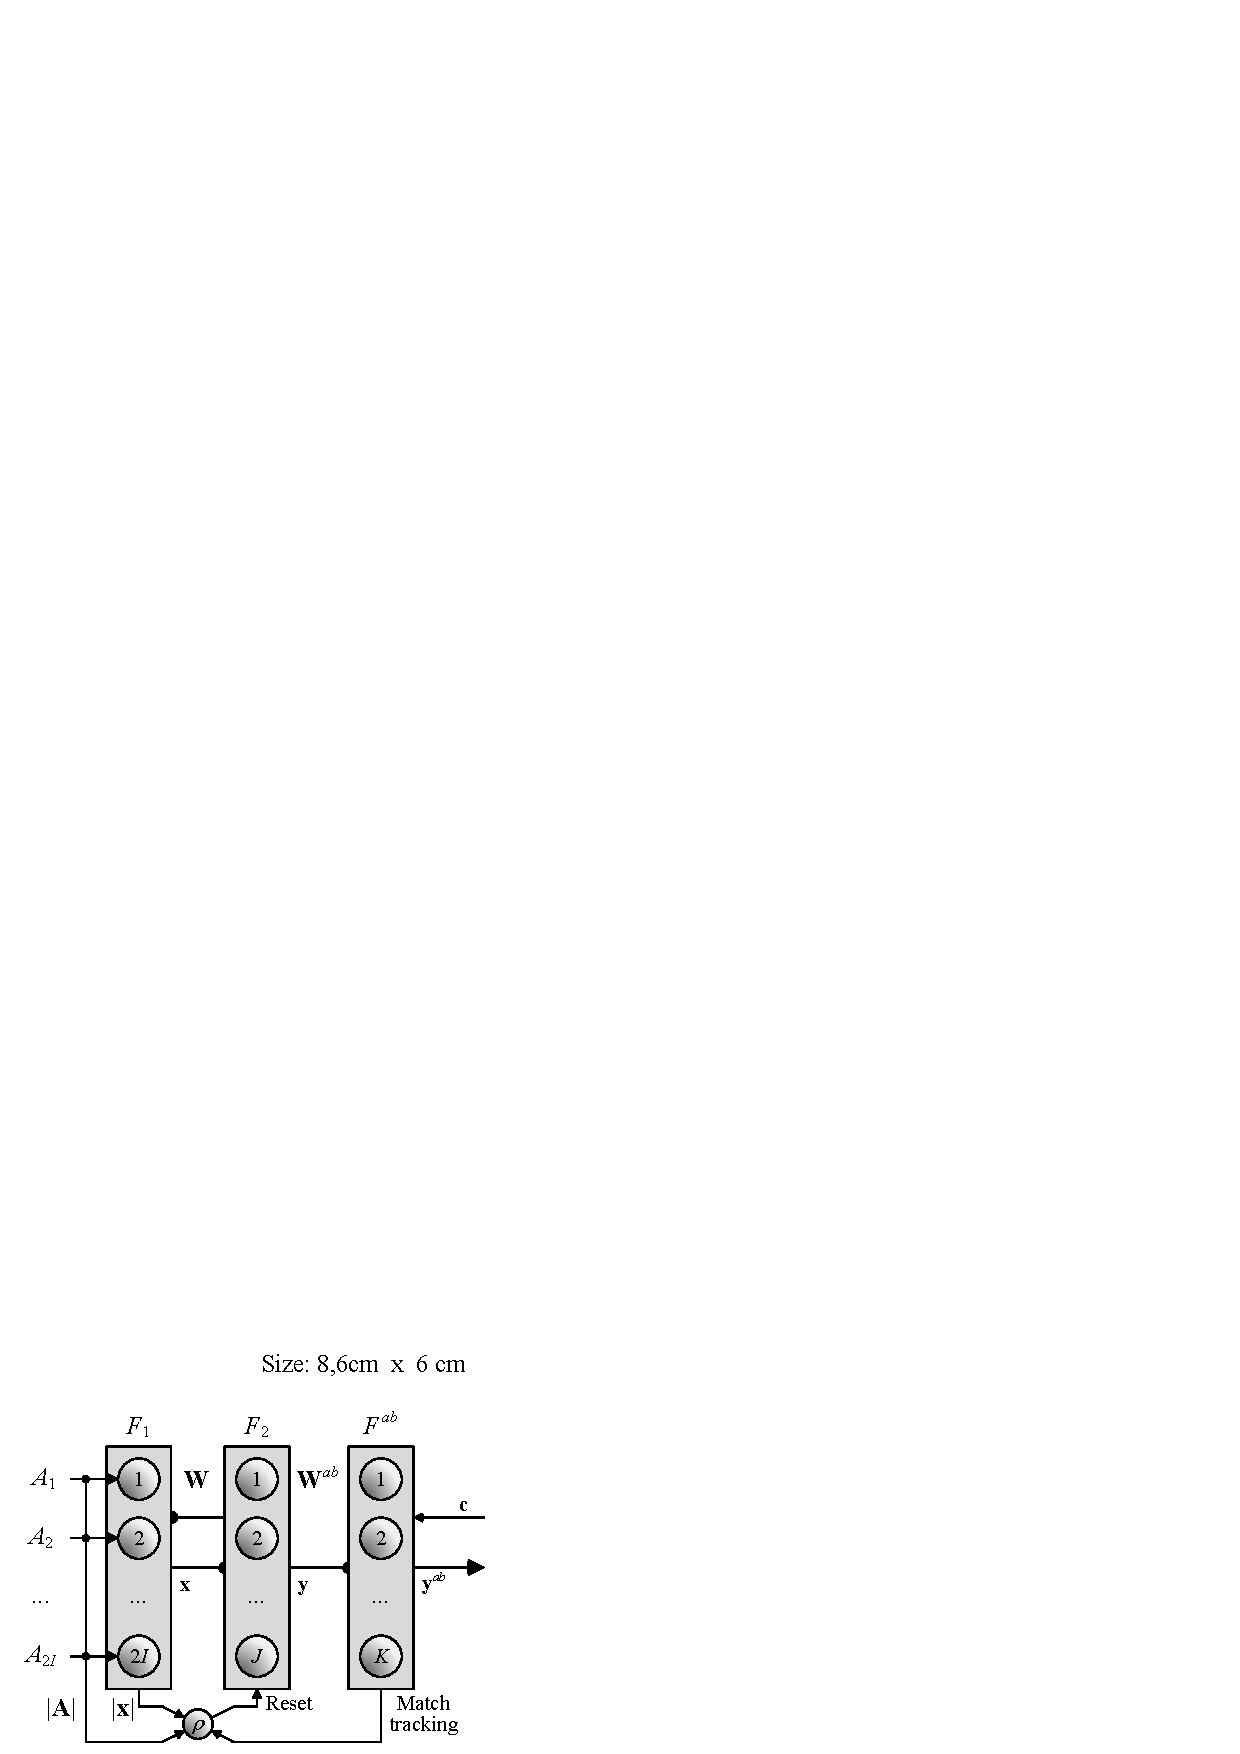
\includegraphics[width=0.5\linewidth, viewport=0cm 0cm 8.6cm 6cm, clip]
  							  {c2_fig3} }
	\caption{Fuzzy ARTMAP neural network}
	\label{fig:c2_fam}
\end{figure*}
%------------------------------- \Fuzzy ARTMAP --------------------------------%

As shown in Figure \ref{fig:c2_fam}, the fuzzy ARTMAP (FAM) architecture consists of three layers: (1) an input layer $F_1$ of $2I$ neurons, with two neurons associated with each input feature (in $\mathbb{R}^I$), (2) a competitive layer $F_2$ of $J$ neurons, each one associated to a recognition category in the feature space, and (3) a map field $F^{ab}$ of $K$ output neurons, each one corresponding to a class (\cite{carpenter92}).

In supervised training mode, FAM learns an arbitrary mapping between training set patterns $\textbf{a}$ = $(a_1, a_2, ..., a_I)$ and their corresponding binary supervision patterns $\textbf{c}$ = $(c_1, c_2, ..., c_K)$.
These patterns are coded to have the value $c_k = 1$ if $k^*$ is the target class label for $\textbf{a}$, and zero elsewhere.
Components of the vector $\textbf{a}$ are scaled so that each $a_i \in [0,1]$, for $i=1 \ldots I$.
Complement coding doubles the number of components in the input vector, which becomes $\textbf{A} \equiv (a_1, a_2, ..., a_I, 1-a_1, 1-a_2,..., 1-a_I)$.
The prototype vector $\textbf{w}_{j} = (w_{1j}, ..., w_{2Ij})$, linking each $F_1$ input node to $F_2$ node $j$, may be visualized as a hyper-rectangle in the $\mathbb{R}^I$ feature space defined by all the input vectors $\textbf{a}$ that selected node $j$ during training.
Binary weight vectors $\textbf{w}^{ab}_{j} = (w_{j1}, ..., w_{jK})$ connects $F_2$ nodes to one of the $K$ classes of $F^{ab}$.

Initially, all the $F_2$ nodes are uncommitted, all weight values $w_{ij}$ are initialized to 1, and all weight values $w^{ab}_{jk}$ are set to 0.
Prior processing each new training pattern $\textbf{a}$, the vigilance parameter is set: $\rho=\bar{\rho}$.
Given an input $\textbf{a}$ and supervision output $\textbf{c}$, the coding field $F_2$ is activated according to the Weber law choice function:
\begin{equation}
	T_j(\textbf{A}) = |\textbf{A}\wedge\textbf{w}_{j}| / (\alpha + 			
										|\textbf{w}_{j}|),
	\label{eq:choice}
\end{equation}
where $(\textbf{p}\wedge\textbf{q})_i \equiv \textrm{min} (p_i,q_i)$, $|\textbf{p}| \equiv \sum^{2I}_{i=1} |p_i|$, and $\alpha$ is the \emph{choice parameter}.
With winner-take-all coding, the $F_2$ node $j^*$ that receives the largest activation $T_{j^*}(\textbf{A})$ is chosen, and undergoes the vigilance test defined by: 
\begin{equation}
	|\textbf{A}\wedge\textbf{w}_{j^*}| / |\textbf{A}|=|\textbf{A} \wedge 
		\textbf{w}_{j^*}|/I > \rho,
	\label{eq:match}
\end{equation}
where $\rho \in [0,1]$ is the dimensionless \emph{vigilance parameter}.
If node $j^*$ passes the vigilance test, FAM predicts the class corresponding to $j^*$.
If the prediction is correct (\emph{i.e.}, $k(j^*)=k^*$), weight vector $\textbf{w}_j$ undergoes learning and is adjusted according to
\begin{equation}
  \textbf{w}_{j^*}' = \beta(\textbf{A} \wedge \textbf{w}_{j^*}) + 
   										(1 - \beta) \textbf{w}_{j^*} \,,
  \label{eq:learning}
\end{equation}
where $\beta \in [0,1]$ is a fixed \emph{learning rate parameter}.

If neuron $j^*$ does not pass the vigilance test, or makes an \emph{incorrect} class prediction, it is deactivated for the rest of the search process with the current input $\textbf{a}$.
When an incorrect class prediction occurs, a \emph{match tracking} signal also adjusts vigilance such as $\rho = |\textbf{A} \wedge	\textbf{w}_{j^*}|/I + \epsilon$, where $\epsilon$ is the match tracking parameter.\footnote{In this chapter, negative match tracking is employed (\cite{carpenter98}).}
The network then searches for another $F_2$ node that either satisfies both requirements, or commits a new $F_2$ node to encode $\textbf{a}$ if no such node exist.
When a new $F_2$ node is committed, network size is actualized ($J=J+1$), and the last committed node learns the correct output class by setting  $\textbf{w}_J = \textbf{A}$ and $w^{ab}_{Jk^*} = 1$.

During training, FAM internal dynamics are governed by four hyperparameters: the choice parameter $\alpha \geq 0$, the learning parameter $\beta \in [0,1]$, the match tracking parameter $\epsilon \in [-1,1]$, and the baseline vigilance parameter $\bar{\rho} \in [0,1]$.
Let $\textbf{h}=(\alpha, \beta, \epsilon, \bar{\rho})$ be defined as the vector of FAM hyperparameters, these are inter-related and each have a distinct impact on network dynamics.
While $\alpha$ and $\epsilon$ determine the depth of search attained before an uncommitted node is selected, and $\bar{\rho}$ limits the maximal size of the category hyper-rectangles in the $\mathbb{R}^I$ feature space.
Although this is affected by the match tracking signal $\epsilon$, low baseline vigilance generally results in large hyper-rectangles and leads to broad generalization and abstract memories, while high vigilance yields small hyper-rectangles, leading to narrow generalization and detailed memories.
During learning, $\beta$ determines the speed with which the recognition categories expand to fit $\textbf{a}$.
The algorithm can be set to slow learning with $0<\beta<1$, or to fast learning with $\beta=1$.
With fast learning, each hyper-rectangles is just large enough to enclose the training set patterns $\textbf{a}$ to which it has been assigned.
Prototype vector $\textbf{w}_j$ records the largest and smallest component values of training subset patterns $\textbf{a}$ assigned to category $j$.

A standard vector of hyperparameters $\textbf{h}_\text{std} = (\alpha = 0.001, \beta=1, \epsilon=0.001, \bar{\rho}=0)$ is commonly fixed to minimize network complexity (\cite{carpenter92}).
However, Figure 4 illustrates with a synthetic 2D data base (\cite{valentini03}) that adjusting these hyperparameters allows to adapt FAM learning dynamics with regards to currently available training data.
By using different hyperparameters settings to train FAM, each network learns different hyper-rectangles to fit the same data, leading to different decision boundaries and predictions.
This diversity of opinion among classifiers may then be measured using several different indicators (\cite{canuto07, hadjitodorov06, kapp07, oliveira09, sirlantzis08, ulas09}).

It is very well known that ensembles of classifiers can be used to improve the generalization capabilities of pattern recognition systems applied in different domains, including face recognition in video (\cite{er02, lu06, su07}).
But as Figure 4 shows, varying the hyperparameter values of several FAM neural networks provides an easy mean to model the same data with different perspective and generate a diversified pool of heterogeneous classifiers when few learning reference data is available. 
Given this correlation between diversity of hyperparameter values and decision boundaries, classifier diversity can also be easily exploited during ensemble selection form the pool to further improve accuracy of the face recognition system (\cite{brown05}).

%-------------------------- P2 data & FAM boundaries --------------------------%
\begin{figure*}[t]
  \centering
  \fbox{
		\subfloat[Original data]{
		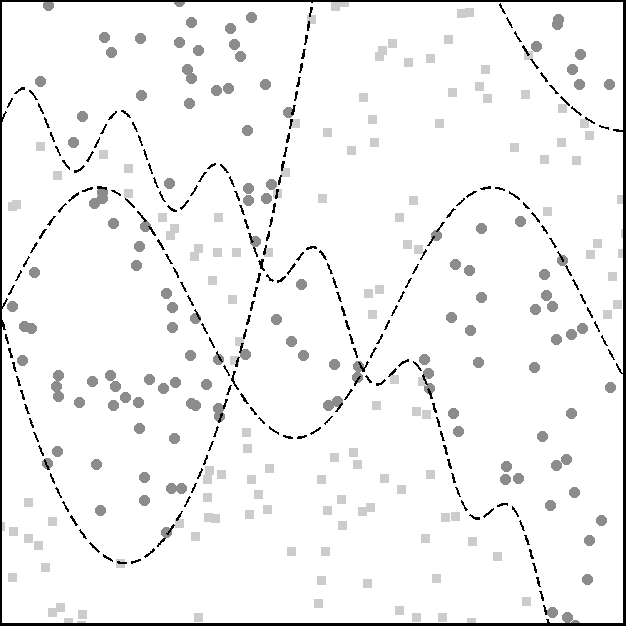
\includegraphics[width=0.22\linewidth]{c2_fig4a} \label{fig:c2_dbp2} }
		\quad
		\subfloat[FAM decision boundaries]{
			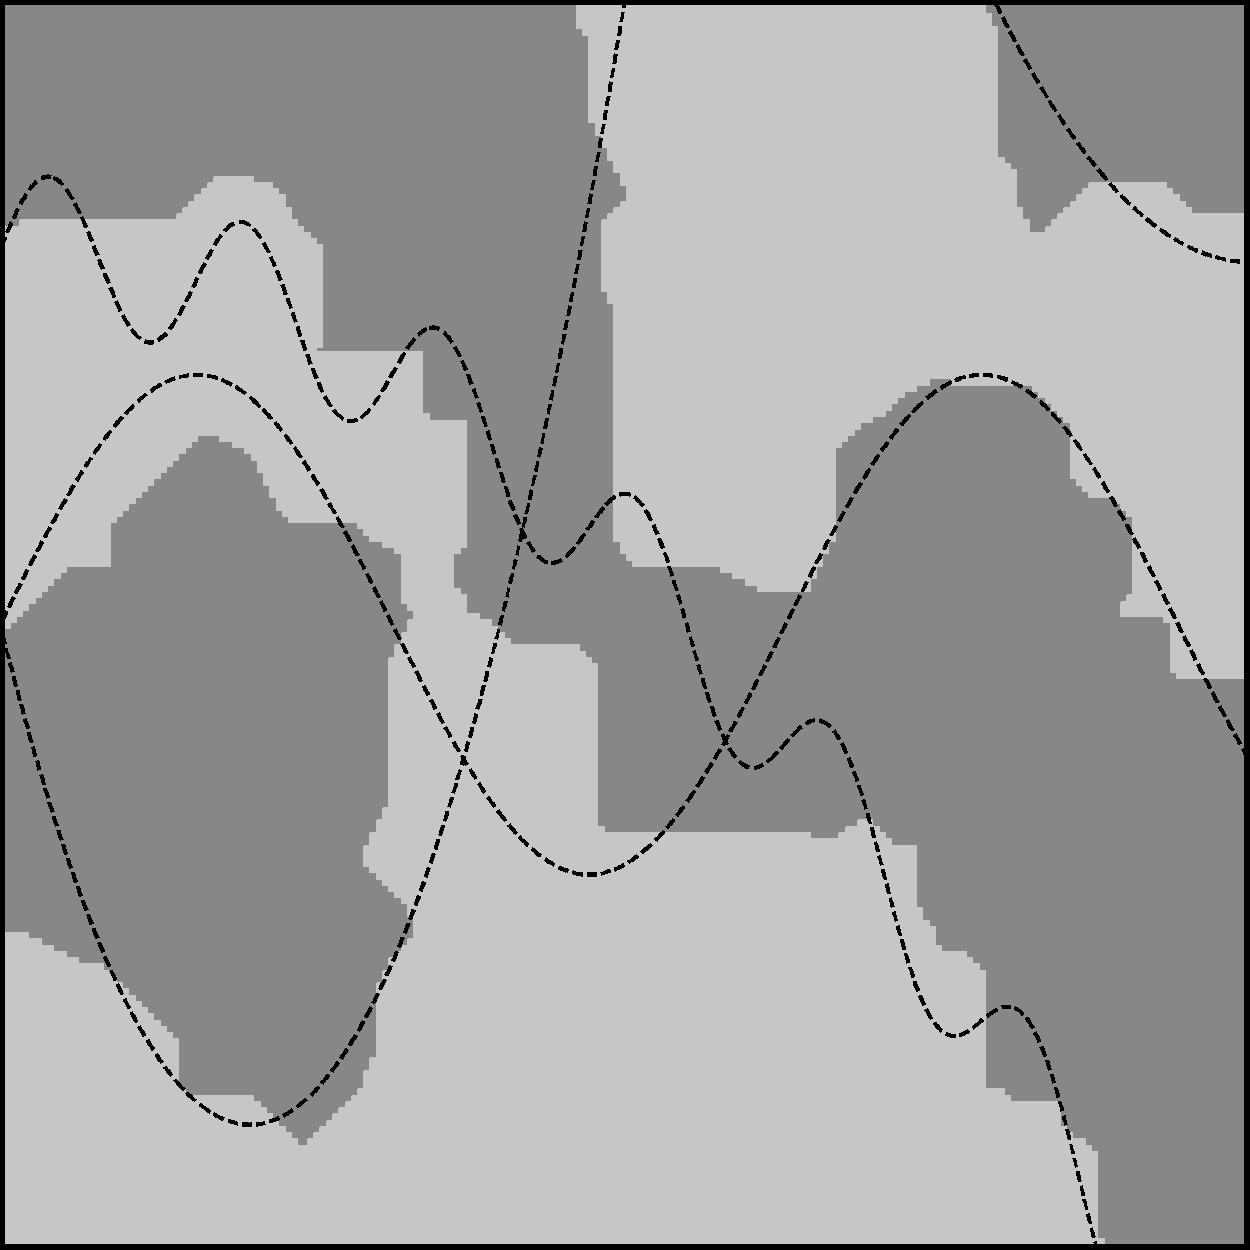
\includegraphics[width=0.22\linewidth]{c2_fig4b} 
			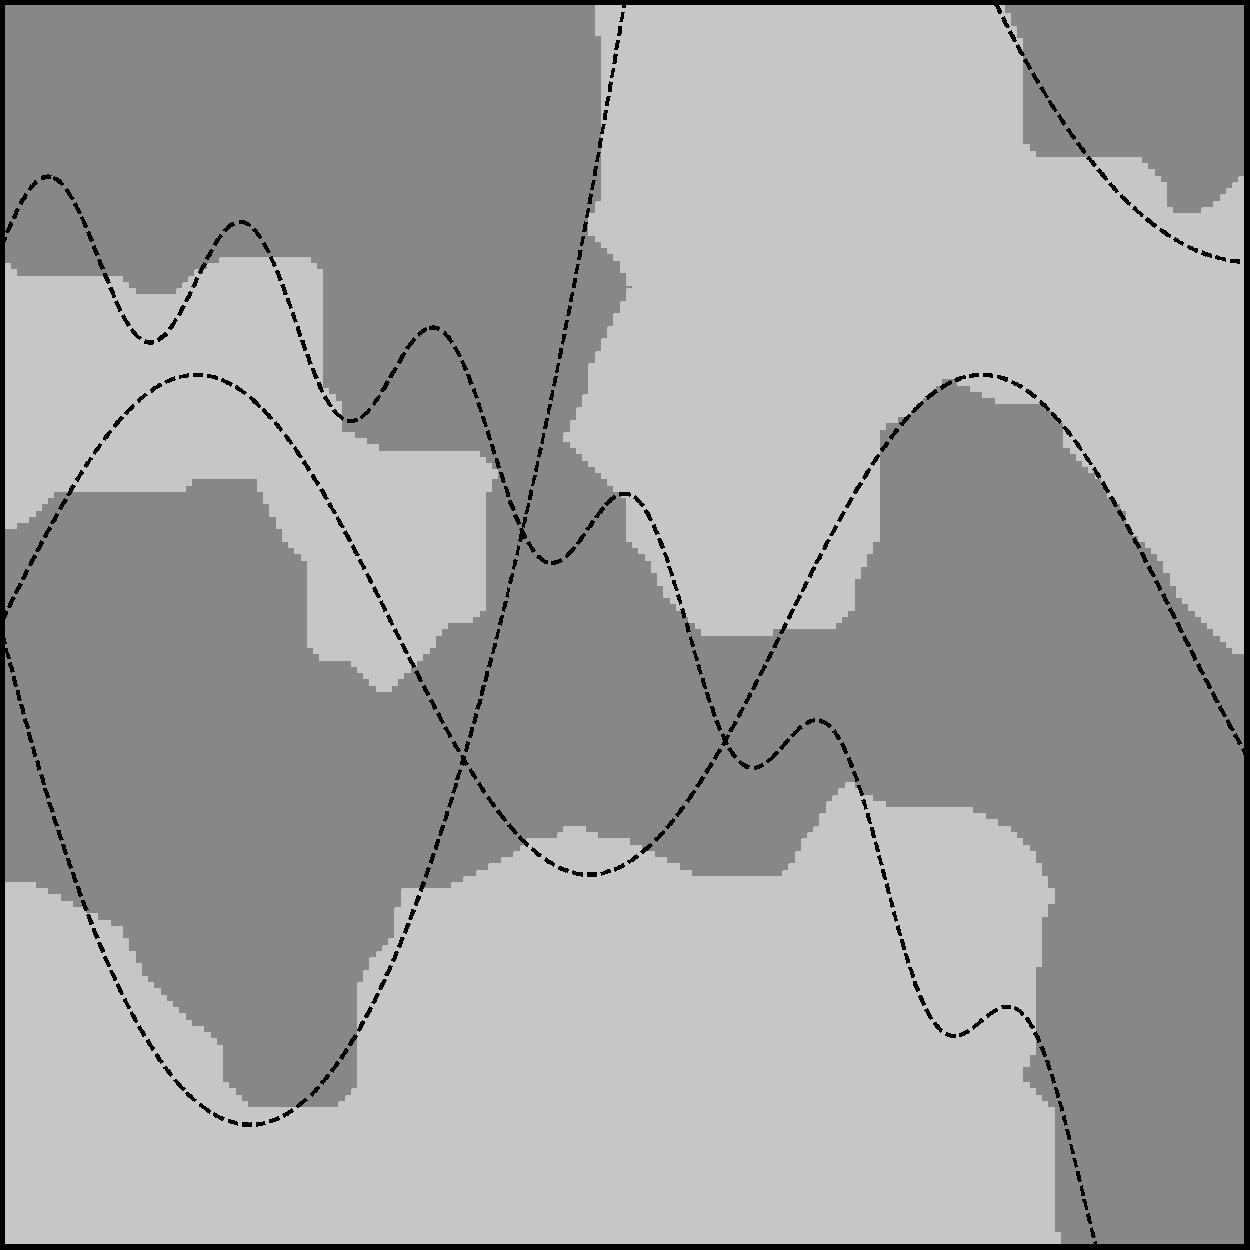
\includegraphics[width=0.22\linewidth]{c2_fig4c} 
			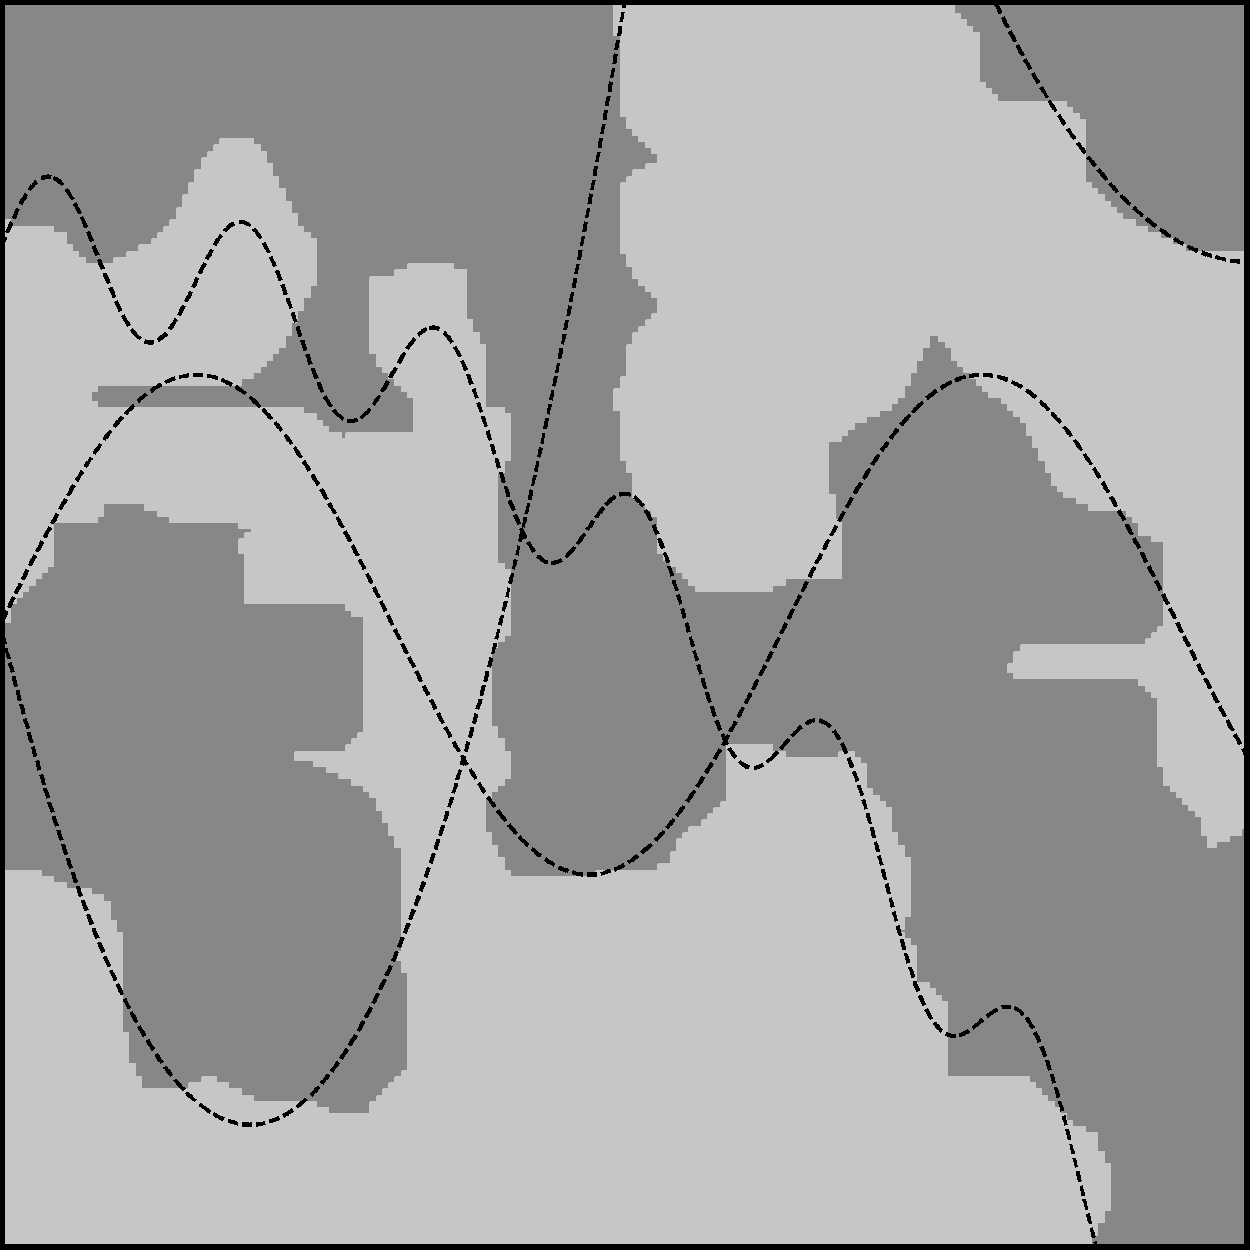
\includegraphics[width=0.22\linewidth]{c2_fig4d}
			\label{fig:c2_famBound}
		}
	}
  \caption{Training data (\ref{fig:c2_dbp2}) from the P2synthetic data base (\cite{valentini03}), and decision boundaries for FAM trained with different hyperparameters that are respectively (\ref{fig:c2_famBound}): $\textbf{h}=($70, 0.70, 0.80, 0.85), $\textbf{h}=($13, 0.41, 0.08, 0.86), and $\textbf{h}=($67, 0.73, 0.68, 0.89)}
	\label{fig:c2_bound}
\end{figure*}
%------------------------- /P2 data & FAM boundaries --------------------------%

%------------------------------------------------------------------------------%
%------------------------------ subsection : pso ------------------------------%
\subsection{Dynamic particle swarm optimization}
\label{sec:c2_dpso}

Particle swarm optimization (PSO) is a population-based stochastic optimization technique that was inspired by social behavior of bird flocking and fish schooling.
With PSO, each particle corresponds to a single solution in the hyperparameter space, and the population of particles is called a swarm.
Particles move through the hyperparameter space and change their course under the guidance of a cognitive influence (i.e., their own previous search experience) and a social influence (i.e., their neighborhood previous search experience).
Unlike evolutionary algorithms (like genetic algorithms), each particle always stores its best position and the best position of its surroundings in its memory.

Originally developed for static optimization problems, the PSO algorithm has been adapted for dynamic optimization problems by adding mechanisms to (1) modify the social influence to maintain diversity in the optimization space and detect several optima, (2) detect changes in the objective function by using the memory of each particle, and (3) adapt the memory of its population if change occur in the optimization environment.
The latest particle swarm optimization algorithms developed to insure diversity in the swarm are presented in \cite{du08, li06, nickabadi08_2, ozcan07}.
Change detection and memory adjustment mechanisms for DPSO are presented in \cite{blackwell04, carlisle02, hu02, wang07}.

During supervised incremental learning of new data blocks $D_t$, the dynamic optimization module (see Figure 2) iteratively updates the hyperparameter vector $\textbf{h}=\left(\alpha, \beta, \epsilon, \bar{\rho}\right)$ of each FAM classifier in the hyperparameter space, and determines the position $\textbf{h}$ such that the FAM classification rat is maximized.
In this chapter, the hyperparameter space is bounded by $\alpha \in \left[0,100\right]$, $\beta \in \left[0,1\right]$, $\epsilon \in \left[-1,1\right]$, and $\bar{\rho} \in \left[0,1\right]$.
Using PSO to evolve a swarm of FAM networks when data is learned incrementally over time, such adaptation has been shown to correspond to a dynamic optimization problem defined by  
\begin{equation}
	\textnormal{maximize }\{ f(\textbf{h},t)\ |\ \textbf{h}\in\mathbb{R}^4,
																             \ t\in\mathbb{N}_1 \},
	\label{eq:optDyn}
\end{equation}
where the fitness, $f(\textbf{h},t)$, is the FAM classification rate for a given vector of hyperparameters $\textbf{h}$, and after learning data set $D_t$ at a discrete time $t$ (\cite{connolly10}).
There are three different types of dynamic optimization environment (\cite{engelbrecht05}): type I, where the location of the optimum changes over time; type II, where the location of the optimum remains fixed, but the value of the objective function optimum's position changes; and type III, where both the location and value of the optimum position change.
In \cite{connolly10}, it was shown that the optimization problem defined by Equation \ref{eq:optDyn} constitute a type III optimization environment.

%-------------------- DNPSO - subswarms and free particles --------------------%
\begin{figure*}[t]
  \centering
  \fbox{
		\subfloat[$t=1$]{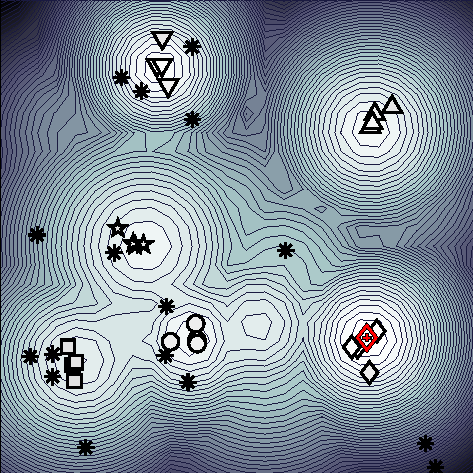
\includegraphics[width=0.23\linewidth]{c2_fig5a}}
		\hspace{1mm}
		\subfloat[$t=2$]{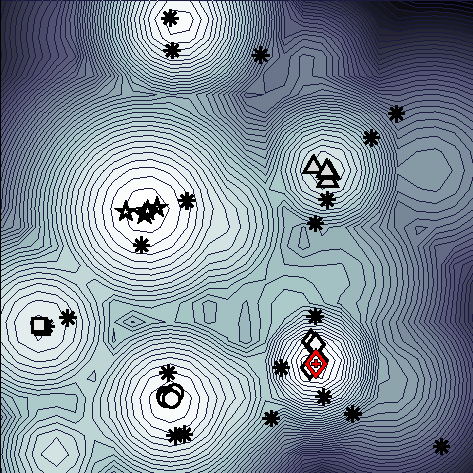
\includegraphics[width=0.23\linewidth]{c2_fig5b}}
		\hspace{1mm}
		\subfloat[$t=3$]{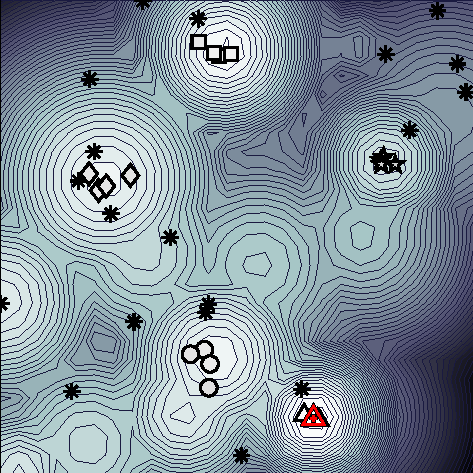
\includegraphics[width=0.23\linewidth]{c2_fig5c}}
		\hspace{1mm}
		\subfloat[$t=4$]{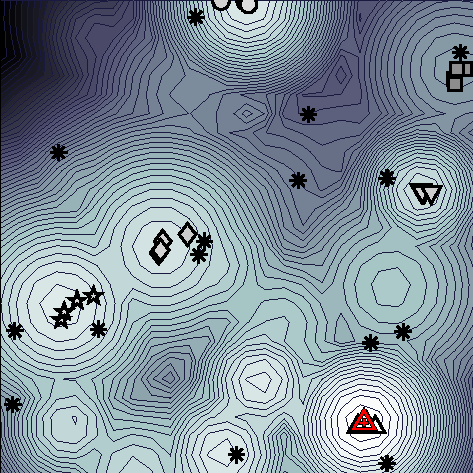
\includegraphics[width=0.23\linewidth]{c2_fig5d}}
	}
	\caption{Evolution of DNPSO particles for different changes in a type III 
optimization environment using the 2D multipeak benchmark problem (\cite{branke99}).
In a video-based face recognition application for instance, this could be the classification rate landscape in a 2D hyperparameter space.
Subswarms (shapes: circle, rectangle, etc.) are created dynamically around the \emph{masters} -- particles that detected local optima.
Subswarms converge toward the local optima detected for the objective function.
Free particles (stars), that are not associated to any subswarms, are free to explore the optimization space using only their cognitive influence.
At different times $t$, the personal best of each particles is reevaluated to accommodate changes that may occur on the objective function}
	\label{fig:c2_dnpso}
\end{figure*}
%------------------- /DNPSO - subswarms and free particles --------------------%

In this chapter, the adaptive multiclassifier system (AMCS) employs the Dynamical Niching PSO (DNPSO) algorithm (\cite{nickabadi08_2}) to maximize FAM classification rate as a function of its hyperparameters.
As depicted in Figure \ref{fig:c2_dnpso}, this algorithm maintains diversity in the hyperparameter search space by (1) using a local neighborhood topology, where subswarms are dynamically created around \emph{masters} (particles that are their own local best in their neighborhood), by (2) defining a minimal distance within which two masters that cannot co-exist, by (3) allowing free particles that do not belong to a subswarm, to move independently, and by (4) reinitializing those free particles that exhibit low velocities, indicating that they have converged on a non-optimal position.
DNPSO has also been adapted for dynamic optimization problems by updating the fitness of the best position of each particle at each iteration.
Using the moving peaks benchmark, the DNPSO algorithm has been shown to detect local optima and converge toward the global maximum in a multimodal type III optimization environment (\cite{nickabadi08_2}) (see Figure \ref{fig:c2_dnpso}).

When evolving FAM neural networks, updating the fitness of the best position of each particle at each iteration would double the number of time each network are trained, leading to a very costly process.
However, for an AMCS, changes in the objective function may only occur when a new data block $D_t$ becomes available.
Thus, the best position's fitness of each particle is only updated when a new $D_t$ is presented to the system, \emph{before} the iterative DNPSO process.

%------------------------------------------------------------------------------%
%------------- subsection: Heterogeneous Ensemble of FAM Networks -------------%
\section{Strategy for evolving heterogeneous ensemble of FAM networks}
\label{sec:c2_algo}

The DPSO-based incremental learning strategy proposed in this chapter is based on the hypothesis that maintaining diversity among particles in the optimization environment implicitly generates diversity among classifiers in the classification environment.
By associating each classifier of a pool to a particle in a swarm, properties of a DPSO algorithm (to maintain diversity in the hyperparameter space) may be exploited to evolve a diversified heterogeneous ensembles of FAM networks over time, as new data becomes available.

This section describes the DPSO-based incremental learning strategy used to evolve heterogeneous ensembles of classifiers in response to new labeled reference samples.
First, a diversified pool of FAM networks is generated and evolved according to a DPSO learning algorithm (Section \ref{sec:c2_pool}).
This pool (or swarm) allows for efficient selection and fusion of ensembles of classifiers based on FAM accuracy and particle swarm diversity in the hyperparameter space (Section \ref{sec:c2_sel}).


%--------------------- subsection: DPSO learning strategy ---------------------%
\subsection{Generation and evolution of heterogeneous classifier pools}
\label{sec:c2_pool}

Algorithm \ref{alg:c2_pso} describes the DPSO algorithm proposed to generate and evolve a diversified pool (or swarm) of $N$ FAM networks.
During incremental learning of a data block $D_t$, their hyperparameters, parameters and architecture are cojointly optimized such that the classification rate is maximized.
For a PSO algorithm with $n=1, ..., N$ particles, each a hyperparameter vector (noted $\textbf{h}_n$), a total of $2N+1$ FAM networks is required.
The system stores $n=1, ..., N$ networks $\textit{FAM}_n^\text{start}$ in a short term memory to preserve networks associated with the best position of each particle (noted $\textbf{h}^*_n$) at time $t-1$.
It also stores $\textit{FAM}_n$, the model associated with $\textbf{h}^*_n$ during the optimization process at time $t$, and $\textit{FAM}_\text{est}$, a network employed for fitness estimation.
To minimize the impact of pattern presentation order at a time $t$, FAM networks are trained using the training data set $D_t^\text{t}$ under five different random pattern presentation orders.
To determine the number of training epochs, cross-validation is performed with the validation data set $D_t^\text{v}$, while fitness is estimated using the fitness estimation data set $D_t^\text{f}$ (\cite{connolly10}).
Overall fitness is defined as the highest classification rate achieved over the five pattern presentation orders, and $\textit{FAM}_\text{est}$ is the network that yields this highest classification rate.

%------------------------------ Algorithm : pso -------------------------------%
\begin{algorithm*}[t]
	\caption{DPSO learning algorithm}
	\label{alg:c2_pso}
 	\fbox{\begin{minipage}{0.97\linewidth}\centering
	\begin{algorithmic}[1]
		\Require New data sets $D_t$ for learning.
		\Ensure  Pool (or swarm) of $N$ FAM networks $\textit{FAM}_n$.
						
		\Statex\vspace{6pt}\textbf{Initialization:}\vspace{3pt}
		\State  $\bullet$ Set the swarm's parameters,                             
		\Statex $\bullet$ Initialize all $N$ networks $\textit{FAM}_{n}$ and
					 					  $\textit{FAM}_n^\text{start}$,
		\Statex	$\bullet$ Set PSO iteration counter at $\tau=0$, and              
		\Statex	$\bullet$ Randomly initialize particles positions and velocities. 
					 																									\label{l:c2_init}
		%-- For each learning block
		\Statex\vspace{9pt}\textbf{Upon reception of a new data block $D_t$, the
					 following incremental process is initiated:}\vspace{3pt}
					 
			%-- Personal best update
			\Statex\textit{Update the fitness of networks associated to the 
						  personal best positions:}\vspace{3pt}
			
			\For{ each particle $n$, where $ 1 \leq n \leq N$ }		\label{l:c2_pUpdate}
				\State Train and validate $\textit{FAM}_n$ with $D_t^\text{t}$ and
				       $D_t^\text{v}$ respectively, and estimate $f(\textbf{h}^*_n, t)$ 
				       using $D_t^\text{f}$.			                \label{l:c2_trnUpdate}
			\EndFor                                            \label{l:c2_endpUpdate}
			
			%-- Loop iterations
			\Statex\vspace{6pt}\textit{Optimization process:}\vspace{3pt}
			\While{ PSO does not reach stopping condition }						\label{l:c2_opt}
				\State Update particle positions according to the DNPSO algorithm.			
																														\label{l:c2_newPos}
				\For{each particle $n$, where $ 1 \leq n \leq N$}		\label{l:c2_fUpdate}
					\State $\textit{FAM}_\text{est}$ $\leftarrow$   \label{l:c2_famUpdate}
								 $\textit{FAM}_n^\text{start}$
					\State Train $\textit{FAM}_\text{est}$ with validation using
								 $D_t^\text{t}$ and $D_t^\text{v}$, and estimate
								 $f(\textbf{h}_n(\tau),t)$ using $D_t^\text{f}$.
								 																						\label{l:c2_trnOpt}
					\If{ $f(\textbf{h}_n(\tau),t) > f(\textbf{h}^*_n,t)$ }																																						\label{l:c2_ifNewP}
						\State \{$\textbf{h}^*_n$, $\textit{FAM}_n$,
										 $f(\textbf{h}^*_n,t)$\} $\leftarrow$ 
									 \{$\textbf{h}_n(\tau)$, $\textit{FAM}_\text{est}$,
									   $f(\textbf{h}_n(\tau),t)$\}				 \label{l:c2_pAssign}
					\EndIf 																				 \label{l:c2_endifNewP}
				\EndFor																					 \label{l:c2_endfUpdate}
				\State $\tau = \tau + 1$											 	 \label{l:c2_itUpdate}
			\EndWhile 																				 \label{l:c2_endOpt}

			\Statex\vspace{6pt}\textit{Define initial conditions for fitness
						 estimation with $D_{t+1}$:}\vspace{3pt}
			\For{ each particle $n$, where $ 1 \leq n \leq N$ }		\label{l:c2_sUpdate}
				\State $\textit{FAM}_n^\text{start}$ $\leftarrow$ $\textit{FAM}_n$
			\EndFor																						\label{l:c2_endsUpdate}
	\end{algorithmic}
	\end{minipage} }
\end{algorithm*}
%------------------------------------------------------------------------------%

During the initialization process (line \ref{l:c2_init}), all the FAM networks are initialized, and the swarm's parameters are set.
Particle positions are then randomly initialized within their allowed range.
When a new $D_t$ becomes available, the optimization process begins.
Fitness associated with the best position of each particle, $f(\textbf{h}^*_n,t)$, is updated according to the new data along with each network $\textit{FAM}_n$ (lines \ref{l:c2_pUpdate}--\ref{l:c2_endpUpdate}).
The optimization process continues were it previously ended until the DNPSO algorithm converges (lines \ref{l:c2_opt}--\ref{l:c2_endOpt}).
The DNPSO algorithm changes the position of subswarms and free particles in the hyperparameter space, and iteratively update each particle's new position along with their fitness (lines \ref{l:c2_newPos}--\ref{l:c2_endfUpdate}).
If new personal best positions are found, the position ($\textbf{h}^*_n$), fitness ($f(\textbf{h}^*_n,t)$), and network associated with the personal best $\textit{FAM}_n$ are updated (lines \ref{l:c2_ifNewP}--\ref{l:c2_endifNewP}).
At each iteration $\tau$, in the cases of equality between $f(\textbf{h}_n(\tau),t)$ and $f(\textbf{h}^*_n,t)$, the network that requires the least resources ($F_2$ nodes) is kept.
Finally, the iteration counter $\tau$ is incremented (line \ref{l:c2_itUpdate}).

Once the DNPSO algorithm converges, the $\textit{FAM}_n$ networks associated to each personal best are stored as $\textit{FAM}_n^\text{start}$ (lines \ref{l:c2_sUpdate}--\ref{l:c2_endsUpdate}).
These networks provide a short term memory of the swarm's state after learning data block $D_{t}$.
When new data becomes available at a time $t+1$, the best network previously obtained at time $t$ ($\textit{FAM}_n^\text{start}$) serves as the initial condition, and is copied to $\textit{FAM}_\text{est}$ prior training on $D_{t+1}$ each time the fitness of particle $n$ is estimated.
For the first learning block $D_1$, the $\textit{FAM}_n^\text{start}$ networks are in an initial state (see Section \ref{sec:c2_fam}).

%--------------------- subsection: Ensemble selection ----------------------%
\subsection{Selection of diversified ensembles}
\label{sec:c2_sel}

Once the pool of classifiers has evolved (Algorithm \ref{alg:c2_pso}), members of this pool are selected to form a heterogeneous ensemble, where each network is trained on the same data, but with different hyperparameters (\cite{valentini03}).
In Algorithm \ref{alg:c2_ens}, DNPSO capabilities to detect several local optima, while maintaining particle diversity in the hyperparameter space, are exploited for a selection of heterogeneous ensembles, driven by accuracy and diversity, that does not require computing costly classifier diversity indicators (\cite{canuto07, hadjitodorov06, kapp07, oliveira09, sirlantzis08, ulas09}).
Indeed, those indicators involve computing the FAM choice functions $T_j(\textbf{A})$ of all the networks over the fitness estimation data set $D_t^\text{f}$. 
In a worse case scenario, the hyperparameter values are set to grow the largest possible FAM network such as $J_n = |D_1^\text{t}\cup ...\cup D_t^\text{t}|$.
Since diversity indicators rely on classifiers disagreements in the decision space, this time complexity is $O(J_n \cdot |D_t^\text{f}| \cdot I)$, where $|D_t^\text{f}|$ is the size of the fitness estimation data set, and $I$ is the number of input features.
In contrast, selecting ensembles in the hyperparameter space represent a less costly approach.
With DPSO algorithms, diversity in the hyperparameter space involves computing the Euclidean distances between the personal best position of each particle.
The time complexity of this operation is $O(N^2)$, where the size of the swarm $N$ is generally smaller than the number of nodes $J_n$, size of the fitness estimation data set $|D_t^\text{f}|$, and the number of input features $I$. 

Prior to selection, the ensemble of FAM networks ($\textit{EoFAM}$) is empty (line \ref{l:c2_initEns}).
Selection is initially performed based on accuracy and diversity (lines \ref{l:c2_ensLocal}--\ref{l:c2_ensLocalEnd}).
During this phase, the ensemble then consists of the networks corresponding to detected local optima in the optimization environment, \emph{i.e.} personal best position of the DNPSO masters.
Not only this ensures that the initial ensemble consist of networks that are locally the most accurate in the swarm, but since DNPSO forces a minimal Euclidean distance between masters, it ensures that this ensemble is also diverse.

%---------------------------- Algorithm : ensemble ----------------------------%
\begin{algorithm*}[t]
	\caption{Ensemble selection based on FAM accuracy and particle diversity}
	\label{alg:c2_ens}
 	\fbox{\begin{minipage}{0.97\linewidth}\centering
	\begin{algorithmic}[1]
		\Require A swarm of $N$ networks associated with DPSO particles.
		\Ensure  A diverse heterogeneous ensemble of FAM networks
		         ($\textit{EoFAM}$).

		\Statex \vspace{6pt}\textbf{Initialization:}\vspace{3pt}
		\State $\textit{EoFAM} \leftarrow \emptyset$ \label{l:c2_initEns}
		
		\Statex \vspace{6pt}\textbf{Selection of the FAM networks associated to
					  detected local optima:}\vspace{3pt}
    \For{$e = 1$ to $N_\text{ss}$, the number of subswarms}\label{l:c2_ensLocal}
			\State $\textit{EoFAM} \leftarrow$ $\textit{FAM}_n$ associated to master
						 particle $e$   
		\EndFor                                             \label{l:c2_ensLocalEnd}

		\Statex \vspace{6pt}\textbf{Second selection aimed to maximize particle
					  swarm diversity using greedy search:}\vspace{3pt}
		\State Compute initial swarm diversity $\overline{\delta_{e_1e_2}}$ for the
					 $N_\text{ss}$ networks in $\textit{EoFAM}$ using Equation
					 \ref{eq:c2_divPso}. 													\label{l:c2_initDiv}

    \For{ $e=1$ to $N-N_\text{ss}$ }										\label{l:c2_greedy}
    	\For{all networks that are not part of ensemble } \label{l:c2_scan}
				\State Find the one that maximizes swarm diversity  
							 $\overline{\delta_{e_1e_2}}$ for the $N_\text{ss}+e$ \\\hspace{36pt}networks in $\textit{EoFAM}$.
			\EndFor																							 \label{l:c2_scanEnd}
			
			\If{ there exist no networks such as $\overline{\delta_{e_1e_2}}$
			     increases, }       
																													 \label{l:c2_ifbetter}
				\State BREAK;																			 \label{l:c2_break}
			\Else
				\State $\textit{EoFAM} \leftarrow$ $\textit{FAM}_n$ associated to the
						particle that maximized $\overline{\delta_{e_1e_2}}$.
																													 \label{l:c2_addNetwork}
			\EndIf
		\EndFor  																						   \label{l:c2_greedyEnd}
	\end{algorithmic}
	\end{minipage} }
\end{algorithm*}
%------------------------------------------------------------------------------%

The second phase of selection seeks to further increase ensemble diversity by using a greedy search that maximizes particle diversity.
For two classifiers $e_1$ and $e_2$, the pairwise diversity between their particles, $\delta_{e_1e_2}$, is defined as the Euclidean distance in the hyperparameter space between those particles.
For \textit{EoFAM}, diversity in the hyperparameter space is then defined by the average value of all Euclidean distances: 
\begin{equation}
  \overline{\delta_{e_1e_2}} = \frac{2}{E (E-1)}
							\displaystyle\sum_{e_1=1}^{E-1} \:
  						\displaystyle\sum_{e_2=e_1+1}^{E} \delta_{e_1e_2},
	\label{eq:c2_divPso}
\end{equation}
where $E$ is the number of networks in the ensemble.
Although computing this particle swarm diversity has a time complexity of $O(N^2)$, it was revealed to be the most accurate (\cite{orlunda08}).
Moreover, compared to training all the FAM network during fitness estimation (in Algorithm \ref{alg:c2_pso}), the computation of $\overline{\delta_{e_1e_2}}$ (Equation \ref{eq:c2_divPso}) is an insignificant component in the overall time complexity.  

Ensemble diversity computed after the first selection process (lines \ref{l:c2_ensLocal}--\ref{l:c2_ensLocalEnd}) and the greedy search is performed (lines \ref{l:c2_greedy}--\ref{l:c2_greedyEnd}).
Algorithm \ref{alg:c2_ens} iteratively scans through all particles that are not part of the ensemble to find those that maximizes swarm diversity $\overline{\delta_{e_1e_2}}$ (lines \ref{l:c2_scan}--\ref{l:c2_scanEnd}).
If no particle can raise diversity, Algorithm \ref{alg:c2_ens} stops (line \ref{l:c2_break}).
Otherwise, the network $\textit{FAM}_n$ associated to the winning particle is added to the ensemble (line \ref{l:c2_addNetwork}).
Although a greedy search is not guaranteed to find the global best solution, it is a monotonic increasing search process that is efficient in practice (\cite{ulas09}).
Greedy search has a time complexity of $O(N^2)$, compared to an exhaustive search that has an exponential time complexity of $O(2^N)$.

Once the selection process is complete, the fusion of responses from selected classifiers is performed using a simple majority vote.
In the case of a tie, simpler FAM networks are favored--the class is predicted by the networks that require the fewest overall number of $F_2$ nodes wins the vote.

%------------------------------------------------------------------------------%
%---------------------- SECTION: Experimental methodology ---------------------%
\section{Experimental methodology}
\label{sec:c2_methodology}

The main problem addressed in this research is the design of accurate and efficient adaptive systems for the classification of faces in video streams.
Biometric systems for the recognition of faces in video streams are relevant in different scenarios, ranging from to open-set video surveillance or screening applications, where criminals or terrorists enrolled to a watch list must be recognized within dense and moving crowds at major events and airports, to closed-set access control applications, where individuals enrolled to system must by identified prior to accessing secured resources.
Other applications involve identification at access control points, verification of laptop or cell phone users, etc.
In this section, a general system for face recognition in video is first described, followed by the data bases, incremental learning
scenarios, and experimental protocol used to evaluated the performances of the proposed DPSO-based incremental learning strategy.
Finally, the protocol employed to analyze the relationship between particle diversity in the hyperparameter space versus classifier diversity in the feature and decision spaces is described, followed by the performance indicators.

%-------------------------- subsection : Application --------------------------%
\subsection{Application--face recognition in video}

It is assumed that 2D images in the video streams of an external 3D scene are captured using one or more IP or network cameras with fast Ethernet interface, and that computer analysis is performed at a distance.
Each camera captures a sequence of 2D images, or frames, from the external scene, and each frame provides the system with a particular view of individuals populating the scene.
First, the system performs segmentation to locate and isolate regions of interest (ROIs) corresponding to the faces in a frame.

From the ROIs, features are extracted for tracking and classification.
The tracking features can be the position in the 2D images, speed, acceleration, and track number assigned to each ROI on the scene (\cite{granger01}).
On the other hand, classifiers will require invariant and discriminant classification features extracted from the ROIs, and mapped to an $\mathbb{R}^I$ input feature space.

The tracking module generally follows the movement or expression of faces across video frames, while the classification module seeks to match input feature patterns to the face models of individuals enrolled to biometric the system.
Biometric matching is typically implemented with a statistical or neural pattern classifier.
With neural network classifiers, for instance, the biometric model of individuals is defined using the hyperparameters, synaptic weights, and architecture (determined in Algorithms \ref{alg:c2_pso}).
Finally, for each video frame, the decision module may combine and accumulate the responses from the tracking and classification modules.
Given a video sequence threshold, and assuming that tracking is ideal, the
frames are presented to the face recognition system and predictions for each ROIs are accumulated over time.
With FAM networks, each prediction consists in a binary vector with one for the predicted class, and zero elsewhere.
After a given number of video frames, prediction for the sequence is the class with the highest accumulated response.
For identification and surveillance applications, the accumulated response is used as a classification score and the result is a list of the most likely or of all possible matching identities, respectively.

%--------------------------- Face recognition system --------------------------%
\begin{figure*}[!t] \centering
  \fbox{
  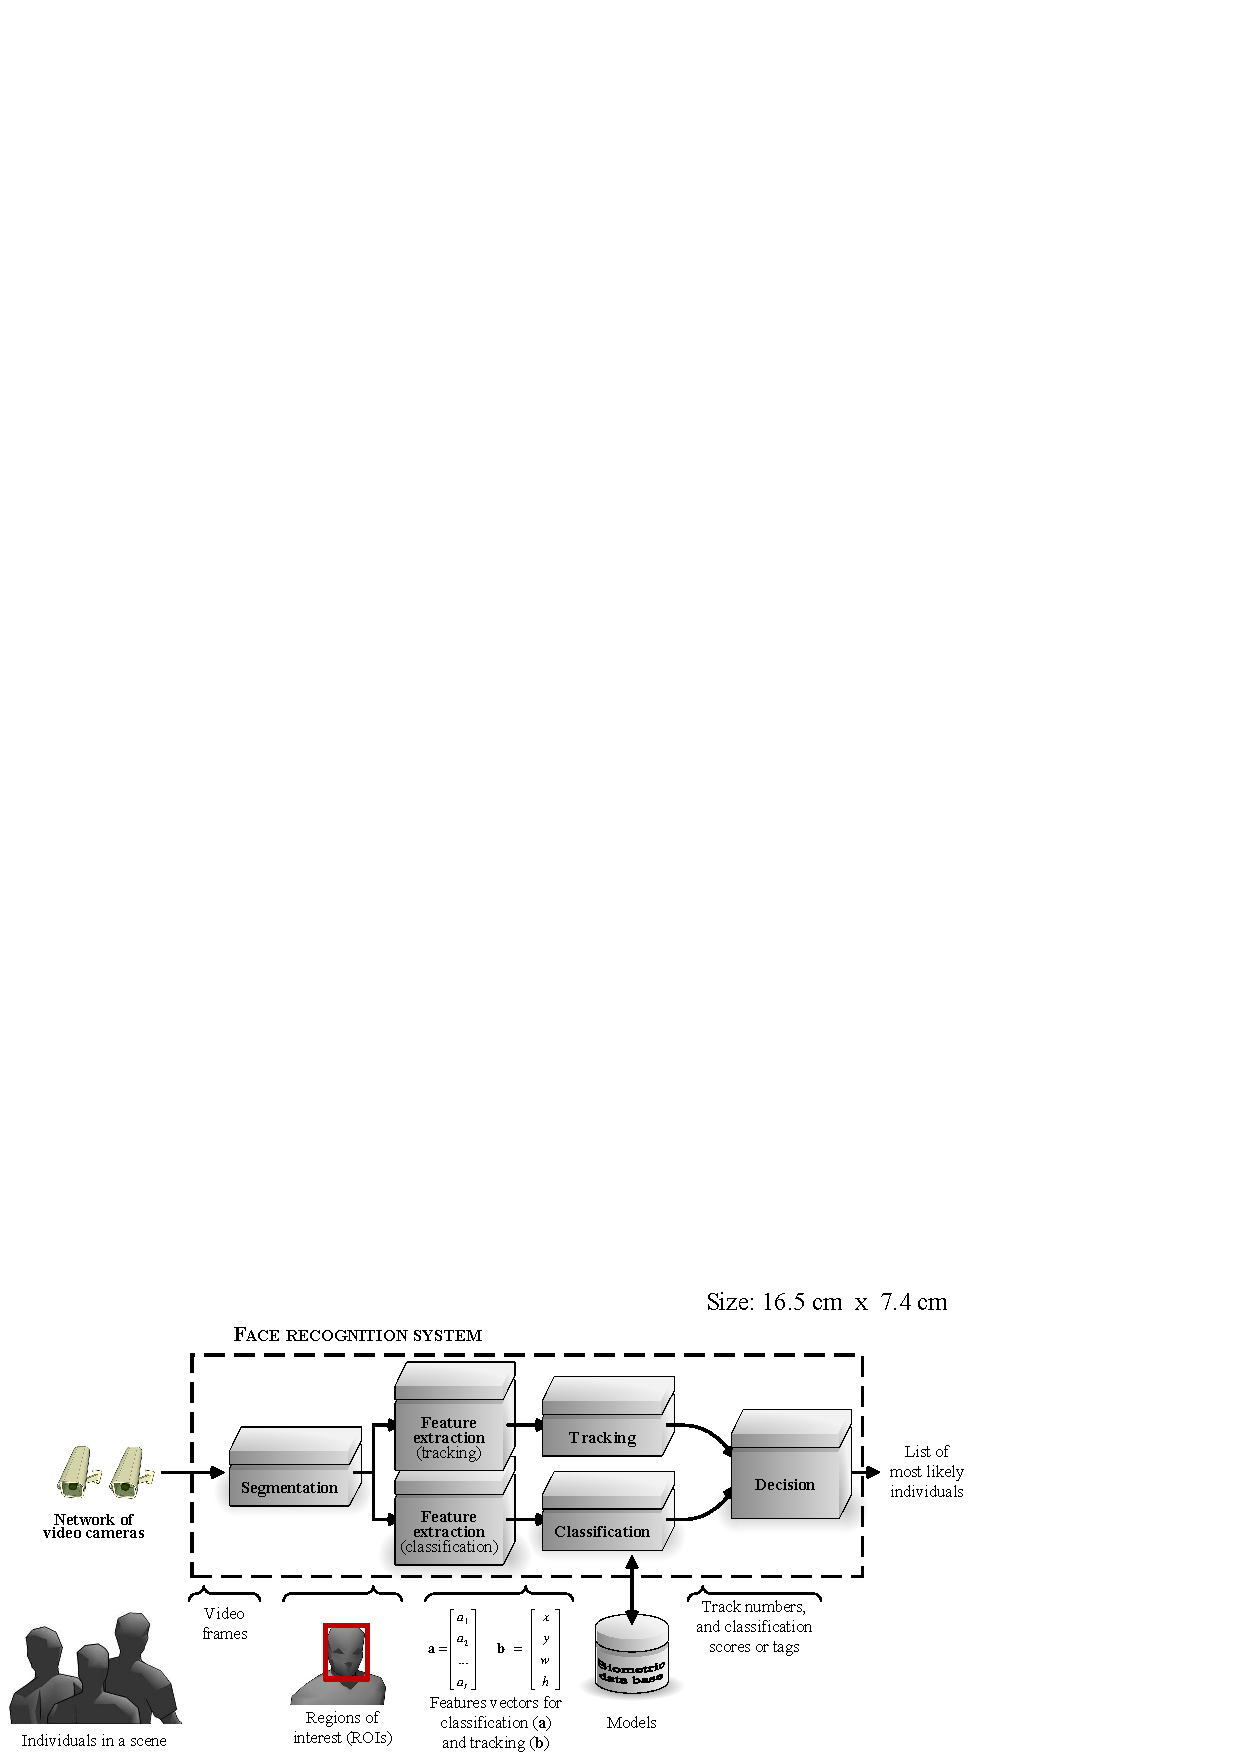
\includegraphics[width=0.97\linewidth, viewport= 0cm 0cm 16.5cm 7.4cm, clip]
 		              {c2_fig6}  }
	\caption{A generic track-and-classify biometric system for video-based face recognition}
	\label{fig:c2_faceRec}
\end{figure*}
%-------------------------- /Face recognition system --------------------------%

Several powerful techniques have been proposed to recognize faces in static 2D images (\cite{zhao03}).
A common approach to recognize faces in video consists in exploiting only spatial information (\emph{i.e.}, appearance), and applying extensions of static image-based techniques on high quality face images produced through segmentation.
The predominant techniques are appearance-based methods like Eigenfaces, and feature-based methods like Elastic Bunch Graph Matching (\cite{zhao03}).
More recently, some authors have exploited temporal information contained in video sequences to improve performance of video-based face recognition.
For example, track-and-classify systems (as the one shown in Figure \ref{fig:c2_faceRec}) combine spatial information with information on motion and appearance of faces in a scene (\cite{connolly10}).
Regardless, the performance of these techniques may degrade considerably when applied in real-world applications.

In addition to difficulties mentioned earlier, video-based face recognition remains a very challenging problem since faces captured in video frames are typically low quality and generally small.
Moreover, there are limitations associated with the camera and techniques used for segmentation, scaling, filtering, feature extraction, and classification (\emph{e.g.}, resolution and noise) (\cite{gorodnichy05, matta09, zhou03}).

%---------------------------- subsection : Database ---------------------------%
\subsection{Video data bases}
\label{sec:c2_db}

In this chapter, experiments are performed by applying AMCS to video-based face recognition in a closed-set access control (identification) applications.
Proof-of-concept simulations are performed with two real-world video data bases for face recognition.

The first data base was collected by the Institute for Information Technology of the Canadian National Research Council (IIT-NRC) (\cite{gorodnichy05}).
It is composed of 22 video sequences captured from eleven individuals positioned in front of a computer.
For each individual, two color video sequences of about fifteen seconds are captured at a rate of 20 frames per seconds with an Intel web cam of a $160\times120$ resolution that was mounted on a computer monitor.
Of the two video sequences, one is dedicated to training and the other to testing.
They are taken under approximately the same illumination conditions, the same setup, almost the same background, and each face occupies between $1/4$ to $1/8$ of the image.
This data base contains a variety of challenging operational conditions such as motion blur, out of focus factor, facial orientation, facial expression, occlusion, and low resolution.
The number of ROIs detected varies from class to class, ranging from 40 to 190 for one video sequences.

The second video data base is called Motion of Body (MoBo), and was collected at Carnegie Mellon University under the HumanID project (\cite{gross02}).
Each video sequence shows one of 25 different individuals on a tread-mill so that they move their heads naturally to four different motion types when walking: slowly, fast, on an inclined surface, and while carrying an object.
Six Sony DXC 9000 cameras, with a resolution of a $640\times480$ pixels, are positioned at different locations around the individuals.
Only the video sequences with visible faces were kept: full frontal view and both sides with an angle of about $70^\circ$ with the full frontal view.

In both cases, segmentation is performed using the Viola-Jones algorithm included in the OpenCV C/C++ computer vision library.
For the IIT-NRC database, the small regions of interest (ROIs) produced are converted in gray scale and normalized to $24\times24$ images where the eyes are aligned horizontally, with a distance of 12 pixels between them.
Principal Component Analysis is then performed to reduce the number of features.
The 64 features with the greatest eigenvalues are extracted and vectorized into $\textbf{a} = \{a_1, a_2, ..., a_{64}\}$, where each feature $a_i \in [0,1]$ are normalized using the min-max technique.
Learning is done with ROIs extracted from the first series of video sequences (1527 ROIs) while testing is done with ROIs extracted from the second series of video sequences (1585 ROIs).
The ROIs obtained with the MoBo data base where processed with Local Binary Pattern and Principal Component Analysis to produce 32 features vectors, also normalized using the min-max technique.
ROIs from sequences for each type of walk and view are divided in two; the first half is used for learning and the second half, for testing.
This yields a total of 36374 learning patterns and 36227 test patterns.
In both cases, the number of features was fixed after error convergence with a 1NN classifier trained on the learning data bases and tested on the test data base.

%------------------------------------------------------------------------------%
\subsection{Incremental learning scenarios}
\label{sec:c2_scenario}

Prior to computer simulations, each video data set is divided in blocks of data $D_t$, where $1\leq t\leq T$, to emulate the availability of $T$ successive blocks of training data to the AMCS during a biometric identification application.
Supervised incremental learning is performed according to two different scenarios.

\subsubsection{Enrollment}

In this scenario, each block contains ROIs of individuals that are not enrolled to the system.
Classes are added incrementally to the system, one at a time.
To assess AMCS performance for $K$ classes, the first learning block $D_1$ is composed of two classes, and each successive block $D_t$, where $2 \leq t \leq K-1$, contains the ROIs captured in a video sequence corresponding to an individual that has not previously been enrolled to the system.
For each $D_t$, performance is only evaluated for existing classes.
To insure the invariance of results to class presentation orders, this experiment is performed using five different random \emph{class} presentation orders.

\subsubsection{Update}

In this scenario, each block contains ROIs of individuals that have previously been enrolled to the system.
It is assumed that at a given time, the ROIs of an individual is captured in a video sequence, and then learned by the system to refine its internal models.
To assess AMCS performance, all classes are initially learned with the first data block $D_1$ and are updated one class at a time with blocks $D_2$ through $D_{K+1}$.
In order to better observe cases where classes are not initially well defined,
block $D_1$ is composed of $10\%$ of the data for each class, and each subsequent block $D_t$, where $2 \leq t \leq K+1$, is composed of the remaining $90\%$ of one specific class.
Here again, invariance to class order presentation is insured by repeating this experimentation with five different \emph{class} presentation orders.

%--------------------- SUBSECTION : Experimental protocol ---------------------%
\subsection{Experimental protocol}
\label{sec:c2_protocol}

To illustrate (1) the performance of Algorithm \ref{alg:c2_pso} with different ensemble selection methods and (2) the impact of diversity in the optimization environment on the models in the classification environment, the results of two experiments are presented in this chapter.
The performance of the proposed DPSO-based learning strategy is first evaluated and compared with various techniques to generate and select classifiers during supervised incremental learning of data blocks $D_t$.
Secondly, the correlation between particle diversity among particles in a swarm (in the hyperparameter) space and diversity among classifiers in an ensemble (in the feature and decision space) is shown empirically .

The DNPSO parameters used for both experiments are shown in Table \ref{tab:c2_pso}.
Weight values $\{w_1,w_2\}$ were defined as proposed in \cite{kennedy07}, and to detect a maximal number of local optima, no constraints were considered regarding the number of subswarms.
Since Euclidean distances between particles are measured with the DNPSO algorithm, the swarm evolves in a \emph{normalized} $\mathbb{R}^4$ space to avoid any bias due to the domain of each hyperparameter.
Before being applied to FAM, particle positions are denormalized to fit the hyperparameters domain.
For each new blocks of data $D_t$, the DPSO optimization process is set to either stop after 10 iterations without improving the classification rate of the best FAM network ($\textit{FAM}_{n^*,t}$) classification rate, or after maximum 100 iterations.

%------------------------------ DNPSO parameters ------------------------------%
\begin{table*}[t]
  \centering
  \caption{DNPSO parameters}
  \begin{tabular*}{\linewidth}{@{\extracolsep{\fill}}|lr|}
  	\hline
	  \textbf{Parameter} & \textbf{Value}     										\\ \hline
		Swarm's size $N$												&  40    						\\
		Weights $\{w_1,w_2\}$ 									&  $\{0.73,2.9\}$ 	\\
		Maximal number of subswarms   					&  $\infty$					\\
		Maximal size of each subswarm 					&  4								\\
		Neighborhood size												&  5    						\\
		Minimal distance between two masters    &  0.1   						\\
		Minimal velocity of free particles    &  0.0001    				\\ \hline
	\end{tabular*}
	\label{tab:c2_pso}
\end{table*}
%------------------------------ \DNPSO parameters -----------------------------%

Learning is performed over ten trials using ten-fold cross-validation with the LTM used as specified in (cite{connolly10}).
The proportion of $D_t$ assign to the LTM, and the maximal number of patterns for each class present in the LTM, are respectively set to $\lambda_D=1/6$ and $|LTM|_k=20$.
Out of the ten folds, eight are dedicated to training ($D_t^\text{t}$), one fold is combined with half of LTM to validate and determine the number of FAM training epochs ($D_t^\text{v}$), and the remaining fold is combined with the other half of the LTM to estimate the fitness of each particle during the DPSO algorithm ($D_t^\text{f}$).
Between successive training epochs, the presentation order of training patterns is changed randomly.
Within each trial, five different replications are performed using different class presentation order, for a total of 50 replications.

The simulations evaluate the performance achieved during both incremental learning scenarios of new data blocks $D_t$, where AMCSs employ the DPSO-based strategy proposed in Section \ref{sec:c2_algo} (Algorithms \ref{alg:c2_pso} and \ref{alg:c2_ens}) to evolve heterogeneous ensemble indicated by LBESTS$_\text{+d}$ (local best particles combined with the diversity greedy search).
This system is compared to AMCSs using the DPSO-based strategy but with different ensemble selection techniques, in particular:
\begin{itemize}
	\item GREEDY$_\text{a}$ $\leftarrow$ the ensemble of FAM networks found using greedy search based on accuracy (\cite{ulas09}),
	\item SWARM $\leftarrow$ the ensemble of FAM networks build with the entire swarm, and 
	\item GBEST $\leftarrow$ the FAM network corresponding to the DPSO global best solution.
\end{itemize}
For references, the performance is also given for an AMCS that uses the entire swarm of FAMs trained with a canonical PSO batch learning strategy (\cite{granger07}) (PSO$_\text{B}$), and a single \textit{k}NN classifier that also performs batch learning.
At a given time $t$, batch learning consist of initializing the system, and learning all the data blocks $D_t$ accumulated so far, $B_t = D_1\cup...\cup D_t$ (\cite{granger07}).

%-------------------------------- Experiment A --------------------------------%
\begin{figure*}[t]
  \centering
  \fbox{
	\subfloat[2D example]   {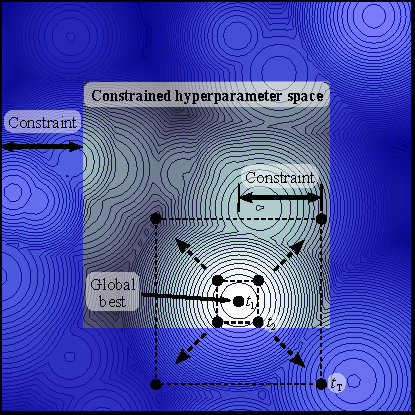
\includegraphics[width=0.44\linewidth]{c2_fig7a}
	         \label{fig:c2_proofEx} }
	\hspace*{10mm}
	\subfloat[2D projection]{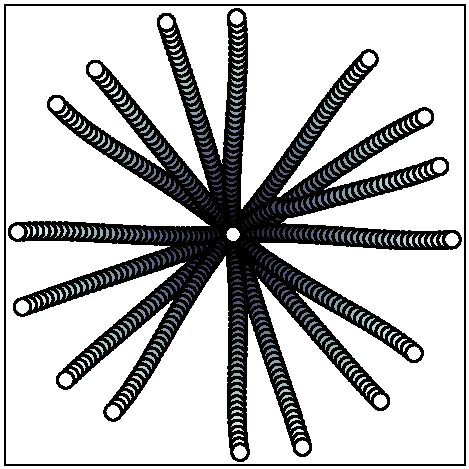
\includegraphics[width=0.44\textwidth]{c2_fig7b}
	         \label{fig:c2_proofPr}	}
	}
  \caption{Example of the particle positions for a 2D objective function (\ref{fig:c2_proofEx}) and 2D projection, obtained using Sammon's mapping of the particle positions in the $R^4$ hyperparameter space (\ref{fig:c2_proofPr}).
The swarm is organized into a hypercube centered around the global best in the in the normalized $R^4$ hyperparameter space.
The hypercube gradually expands, linearly changing particle diversity and affecting the corresponding ensemble of classifiers}
	\label{fig:c2_proof}
\end{figure*}
%------------------------------- \experiment A --------------------------------%

Additional experiments (presented in Figure \ref{fig:c2_proof}) verify the hypothesis under which particle diversity in the optimization environment is correlated to that of ensemble classifier diversity, where each classifier is associated to a particle.
Experiments are performed in two steps: (1) optimization during supervised batch learning of the whole IIT-NRC data base with the DPSO learning strategy, and (2) particles expansion.

Prior to optimization of hyperparameters, the normalized search space is bound by a constraint of 0.2.
Once the global best hyperparameter values are found, an ensemble is formed with 17 FAM networks, each one associated with a particle organized into a hypercube centered around the global best in the normalized $R^4$ hyperparameter space.
One particle is centered at the global best while the other 16 ($2^4$) are positioned as a 4 dimensions hypercube around the center. 
To change the diversity level, all particles are initially situated at the same position of the global best, and the size of the hypercube is gradually expanded up to the value of the constraint to form different swarms (each noted by a different color in Figure \ref{fig:c2_proofPr}).
The expansion of this hypercube will affect a change on diversity in the hyperparameter space.

%--------------------- subsection : performance indicator ---------------------%
\subsection{Performance evaluation and diversity indicator}
\label{sec:c2_indicator}

The average performance of AMCSs is assessed in terms of classification rate over a sequence of one or more ROIs, and resource requirements.
The \emph{classification rate for single facial images (ROIs)} is the ratio of correct predictions over all test set predictions, where each ROIs is tested independently.
Note that classification decisions produced for a single image are considered to be the most conservative performance metric, and it is used for fitness estimation in Algorithms \ref{alg:c2_pso} and \ref{alg:c2_ens}.
However, for the video-based face recognition application, \emph{classification
rate for video sequences} (over two or more ROIs), the result of the fusion between the tracking and classification module, is used.
Given video sequences, it is the ratio of correct predictions over all predictions made by the AMCS accumulated response over a fixed number of video frames.
For unbalanced data bases (\emph{i.e.}, video sequences of different length), classification rate for a number of frames exceeding the length of shorter sequences are computed with predictions obtained with all ROIs of the latter.
The accuracy of AMCSs is also evaluated with cumulative match curves (CMC) (\cite{moon01}).
These curves estimate the ranking capabilities of a classification system for identification applications by providing a cumulative a posteriori probability estimation of having a correct prediction according to rank.

Resource requirements of AMCSs that employ the DPSO learning strategy is measures in terms of \emph{compression}.
That is, the average number of training patterns, contained in all $D_t^\text{t}$ presented to the AMCS, per category prototype in the classifier.
For FAM networks, compression refers to the average number of training patterns per neuron in the $F_2$ layer.
For ensembles, it is the total number of $F_2$ layer nodes for all classifiers in the ensemble.
Since learning with \textit{k}NN consist of memorizing the training data set $D_t^\text{t}$, compression in this case is always one.

While particle swarm diversity is computed using Equation \ref{eq:c2_divPso}, three pairwise indicators are used to compute correlation, or diversity, between two ensemble's classifiers $e_1$ and $e_2$.
As with most measures present in literature, the $Q$ statistic and the correlation coefficient (\cite{ulas09}) rely on classifier disagreement to compute correlation among classifiers.
On the other hand, a specialized ambiguity indicator, inspired by margin theory (\cite{tang06}), is used to compute FAM network diversity.
For two ensemble classifiers $e_1$ and $e_2$, and a given data set (in our case the fitness estimation data set $D_t^\text{f}$), each pairwise indicator is computed as followed:
\begin{enumerate}
	\item \textbf{The $Q$ statistic:}
		\begin{equation} \label{eq:c2_Q}
	    Q_{e_1e_2} \in [0,1] =
	              \frac{N_{11}N_{00}-N_{10}N_{01}}{N_{11}N_{00}+N_{10}N_{01}},
		\end{equation}
where $N_{11}$, $N_{00}$, $N_{10}$, and $N_{01}$ are the number of patterns for each combination of correct and incorrect predictions by classifiers $e_1$ and $e_2$ on the given data set (see Table	\ref{tab:c2_Qstat}).
	\item \textbf{Correlation coefficient:}
\begin{equation}  \label{eq:c2_r}
	\begin{split}
		 \lefteqn{\rho_{e_1e_2} \in [0,1] =}\\
	   & \frac{ N_{11}N_{00} - N_{10}N_{01} }
		{\sqrt{(N_{11}+N_{10})(N_{01}+N_{00})(N_{11}+N_{01})(N_{10}+N_{00}) }},
	\end{split}
\end{equation}
%		\begin{equation}
%		  \rho_{e_1e_2} \in [0,1] = \frac{ N_{11}N_{00} - N_{10}N_{01} }
%		{\sqrt{(N_{11}+N_{10})(N_{01}+N_{00})(N_{11}+N_{01})(N_{10}+N_{00}) }},
%			\label{eq:c2_r}
%		\end{equation}
	\item \textbf{Specialized ambiguity indicator for FAM networks:} Given a pattern $\textbf{a}$, the FAM network selects the $F_2$ winning node $j^*$, corresponding to the highest choice function $T_{j}(\textbf{a})$, and predicts class $k(j^*)$. FAM ambiguity is defined by: 
		\begin{equation}
			\theta_e \in[0,1] = T_{j^*}(\textbf{a}) -
			                \texttt{max}(T_{j}(\textbf{a}), k\neq k^*).
		\end{equation}
Diversity between two FAM classifiers $e_1$ and $e_2$ is defined by the sum of the ambiguity differences for all patterns in the fitness estimation data set ($|D_t^\text{f}|$):
		\begin{equation}
			\Delta\theta_{e_1e_2} \in]0,|D_t^\text{f}|] =
	                   \displaystyle\sum^{|D_t^\text{f}|}
	                   |\theta_{e_1}-\theta_{e_2}|.
			\label{eq:c2_divFam}
		\end{equation}
\end{enumerate}

Ensemble diversity is then defined as the average value deprived from all combination of the pairwise classifier diversity indicators, computed in the same manner as Equation \ref{eq:c2_divPso}. 
Measures from Equations \ref{eq:c2_Q}, \ref{eq:c2_r}, and \ref{eq:c2_divFam} are noted: $\overline{Q_{e_1e_2}}$, $\overline{\Delta \rho_{e_1e_2}}$, and $\overline{\Delta \theta_{e_1e_2}}$.
Higher ensemble diversity is observed for low correlation indicators values ($\overline{Q_{e_1e_2}}$ and $\overline{\Delta \rho_{e_1e_2}}$) and for high values of the FAM diversity indicator ($\overline{\Delta \theta_{e_1e_2}}$).

%--------------------------------- Q statistic --------------------------------%
\begin{table}[t]
  \centering
  \caption{Contingency table used to compute diversity among ensemble classifiers with the $Q$ statistic and correlation coefficient}
  \begin{tabular}{|l|cc|}
  	\hline
  	& $\textit{FAM}_{e2}$ correct & $\textit{FAM}_{e2}$ incorrect \\ \hline
  	$\textit{FAM}_{e1}$ correct   & $N_{11}$ & $N_{10}$ \\ 
  	$\textit{FAM}_{e1}$ incorrect & $N_{01}$ & $N_{00}$ \\ \hline
	\end{tabular}
	\label{tab:c2_Qstat}
\end{table}
%-------------------------------- \Q statistic --------------------------------%

%------------------------------------------------------------------------------%
%------------------------------------------------------------------------------%
%---------------------------- Results & Discussion ----------------------------%
\section{Results and discussion}
\label{sec:c2_results_discussion}

%------------------------------------------------------------------------------%
\subsection{Performance for single images (ROIs)}

To assess the performance of ensembles evolved using the DPSO-based learning strategy, Figures \ref{fig:c2_add} and \ref{fig:c2_upd} present the average classification rate obtained with single facial regions of interest (ROIs), compression, and ensemble size achieved versus the number of data blocks $D_t$.
Results obtained after learning all IIT-NRC and MoBo data bases with both learning scenarios are shown in Tables \ref{tab:c2_add} and \ref{tab:c2_upd}.
For both incremental learning scenarios, results are shown for AMCSs that employs the DPSO-based strategy proposed in Section \ref{sec:c2_algo} (LBESTS$_\text{+d}$).
It is compared to ensembles formed with the entire swarm of FAM networks (SWARM) and the global best network only (GBEST).
In all cases, the accuracy-based greedy search (\cite{ulas09}) (GREEDY$_\text{a}$) is unable to improve the recognition capabilities of the single global best network (GBEST).
Its performances are thus not shown.  
For reference, performance is also shown for batch learning with an ensemble formed with the entire swarm (PSO$_\text{B}$) and the $k$ nearest neighbors algorithm (\textit{k}NN).
For face recognition on single ROIs from the IIT-NRC data base, \cite{arandjelovic09} was able to achieve a classification rate of 91\%, while \cite{gorodnichy05} obtained a classification of 80\%.
In both cases, batch learning was performed with settings in \cite{gorodnichy05}; that is, the features are vectorized as unprocessed gray scale values of the $24 \times 24$ images and one class was used to verify the false acceptance rate rather than the classification rate.
No such results are available for the MoBo data base.

%------------------------------------------------------------------------------%
%----------------------------- Enrollment scenario ----------------------------%

%-------------------------- Result - NRC & enrollment -------------------------%
\begin{figure*}[t]
  \centering
  \fbox{\begin{minipage}{0.97\linewidth}\centering
	\subfloat[]{ 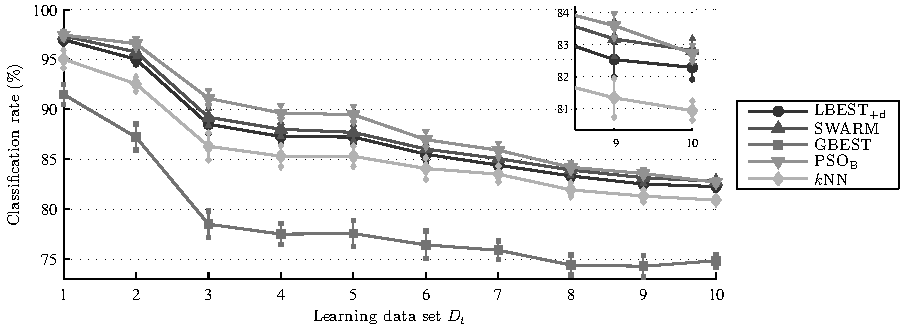
\includegraphics[width=0.95\linewidth]{c2_fig8a} 		 
							 \label{fig:c2_addErr} }  \\
	\subfloat[]{ 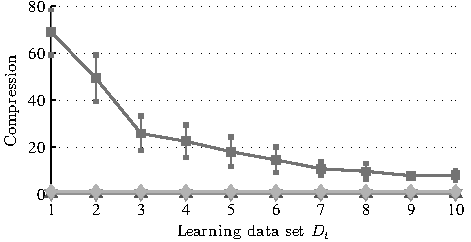
\includegraphics[width=0.47\linewidth]{c2_fig8b}
							 \label{fig:c2_addCpn} }	\quad
	\subfloat[]{ 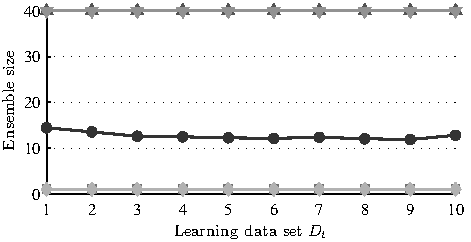
\includegraphics[width=0.47\linewidth]{c2_fig8c}
							 \label{fig:c2_addEns} }
  \end{minipage} }
	\caption{Average classification rate, compression, and ensemble size of the AMCS versus blocks of IIT-NRC data learned during the enrollment scenario.
Performance was evaluated during incremental learning for the AMCS with different ensemble selection techniques and the global best network alone (GBEST).
The performance of the whole swarm optimized during batch learning (PSO$_\text{B}$) and \textit{k}NN are shown for reference.
Error bars correspond to the 90\% confidence interval}
	\label{fig:c2_add}
\end{figure*}
%------------------------- \Result - NRC & enrollment -------------------------%

%---------------------------- Results - enrollment ----------------------------%
\begin{table*}[t]
 \small
 \centering
 \caption{Average classification rate (in percentage), compression and ensemble size after incremental learning of all the IIT-NRC and MoBo data bases for the enrollment scenario.
Each cell is presented with the 90\% confidence interval}
 \begin{tabular*}{\linewidth}{@{\extracolsep{\fill}}|l||rrr||rr|}
 	\hline
		Type of learning &\multicolumn{3}{c||}{Incremental} 
										 &\multicolumn{2}{c|}{Batch} \\ \hline
		Method &\textbf{LBESTS$_\text{+d}$} &SWARM &GBEST &PSO$_\text{B}$ &\textit{k}NN
		\\ \hline
		\multicolumn{6}{|l|}{\vspace{-5pt}}\\
		\multicolumn{6}{|l|}{\hspace{-5pt}\textbf{IIT-NRC data base}}	\\\hline
		Classification rate (\%) & $82.3\pm0.4$     & $82.8\pm0.4$
						 & $74.9\pm0.6$  & $82.7\pm0.2$     & $80.9\pm0.3$  \\
		Compression              & $0.38\pm0.03$    & $0.13\pm0.01$  
						 & $8\pm2$       & $0.062\pm0.003$  & $1\pm0$  			\\
		Ensemble size            & $12.8\pm0.6$     & $40\pm0$
						 & $1\pm0$			 & $40\pm0$         & $1\pm0$  			\\\hline
		\multicolumn{6}{|l|}{\vspace{-5pt}}\\
		\multicolumn{6}{|l|}{\hspace{-5pt}\textbf{MoBo data base}}		\\\hline
		Classification rate (\%) &$92\pm2$       &$91\pm5$
						  &$89.2\pm0.7$  &$94.9\pm0.1$   &$94.5\pm0.1$ 			\\
		Compression              &$1.3\pm0.1$    &$0.48\pm0.02$ 			
						  &$9.0\pm0.9$   &$0.09\pm0.02$  &$1\pm0$  					\\
		Ensemble size   				 &$12.1\pm0.4$   &$40\pm0$
						  &$1\pm0$       &$40\pm0$       &$1\pm0$  					\\\hline
	\end{tabular*}
	\label{tab:c2_add}
\end{table*}
%--------------------------- /Results - enrollment ----------------------------%

For the enrollment scenario, only two classes are present at the beginning of the learning process.
Class decision boundaries are initially simple and classification rates are high.
As classes are added, these boundaries become more complex, leading to a decline in classification rate (see Figure \ref{fig:c2_add}).
When the AMCS is used with the global best only (GBEST), compression also diminishes considerably.
While this is also true when the AMCS uses batch learning (PSO$_\text{B}$), compression and ensemble size for the AMCS with both ensembles methods remains stable during incremental learning.

As expected, after training on all data, GBEST gives the lowest classification rate, while all other solutions give classification rates between 81\% and 83\% (see Figure \ref{fig:c2_add} and Table \ref{tab:c2_add}).
Using LBESTS$_\text{+d}$ gives classification rate comparable to that of SWARM throughout all the enrollment process, except after learning new blocks at times $t=2$ and $t=10$.
However, as compression and ensemble size show (in Table \ref{tab:c2_add}), LBESTS$_\text{+d}$ is able to achieve this accuracy with a third of the resources.

Results with the MoBo data base are consistent with those obtained with the IIT-NRC data (see Table \ref{tab:c2_add}).
However, since position of individuals and video cameras used in the MoBo protocol are fixed, data acquisition is more constrained than with the IIT-NRC data base.
Class distributions are more compact and less likely to vary significantly from one block to the next.
Classification rate and compression follow similar trends excepted that they are generally higher than with the IIT-NRC data base.

%------------------------------------------------------------------------------%
%------------------------------- Update scenario ------------------------------%
%------------------------------------------------------------------------------%
The overall phenomena observed during enrollment resemble the performance observed for the update scenario.
The main difference is that all class distributions are defined from the outset, in $D_1$, and the AMCS initially has knowledge of the entire classification problem.
Due to limited learning data, knowledge of the problem is however incomplete and decision boundaries in the input feature space are then poorly defined, leading to a low classification rate (see Figure \ref{fig:c2_upd}).
As classes are updated incrementally, accuracy of the face recognition system tends to increase.
The highest classification rate are again obtained with LBESTS$_\text{+d}$ and SWARM (Table \ref{tab:c2_upd}).
Although the AMCS with LBESTS$_\text{+d}$ uses about one third of resources used by SWARM, both selection techniques have comparable accuracy over all data blocks, except at times $t=\left\{10,12\right\}$.

%---------------------------- Result - NRC & update ---------------------------%
\begin{figure*}[t]
  \centering
  \fbox{\begin{minipage}{0.97\linewidth}\centering
	\subfloat[]{ 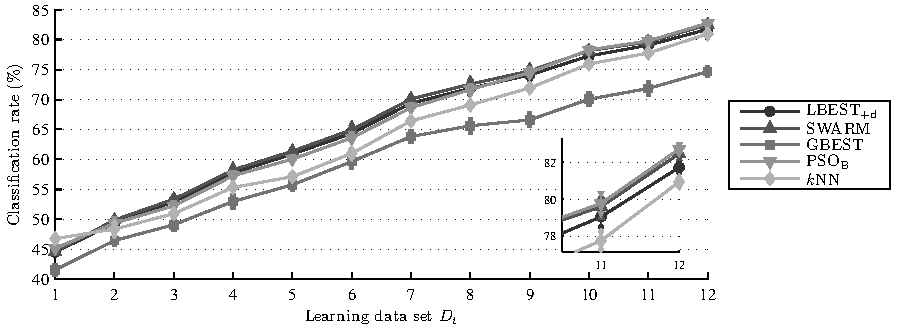
\includegraphics[width=0.95\linewidth]{c2_fig9a}
               \label{fig:c2_updErr} }	\\
	\subfloat[]{ 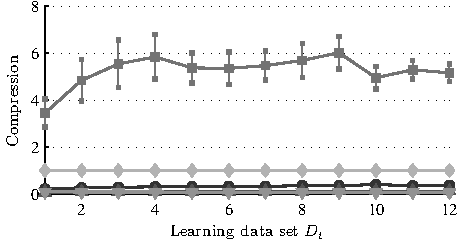
\includegraphics[width=0.47\linewidth]{c2_fig9b}
               \label{fig:c2_updCpn} } \quad
	\subfloat[]{ 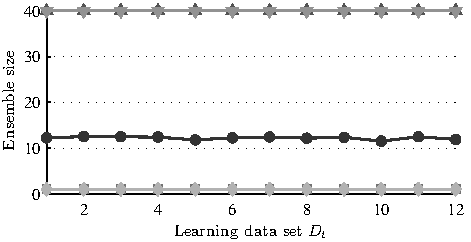
\includegraphics[width=0.47\linewidth]{c2_fig9c}
               \label{fig:c2_updEns} }
  \end{minipage} }
	\caption{Average classification rate, compression, and ensemble size of the AMCS versus blocks of IIT-NRC data learned during the update scenario.
Performance was evaluated during incremental learning for the AMCS with different ensemble selection techniques and the global best network alone (GBEST).
The performance of the whole swarm optimized during batch learning (PSO$_\text{B}$) and \textit{k}NN are shown for reference.
Error bars correspond to the 90\% confidence interval}
	\label{fig:c2_upd}
\end{figure*}
%--------------------------- \Result - NRC & update ---------------------------%

%------------------------------ Results - update ------------------------------%
\begin{table*}[t]
 \small
 \centering
 \caption{Average classification rate (in percentage), compression and ensemble size after incremental learning of all the IIT-NRC and MoBo data bases for the update scenario.
Each cell is presented with the 90\% confidence interval}
 \begin{tabular*}{\linewidth}{@{\extracolsep{\fill}}|l||rrr||rr|}
 	\hline
		Type of learning &\multicolumn{3}{c||}{Incremental} 
										 &\multicolumn{2}{c|}{Batch} \\ \hline
		Method &\textbf{LBESTS$_\text{+d}$} &SWARM &GBEST &PSO$_\text{B}$ &\textit{k}NN
		\\ \hline
		\multicolumn{6}{|l|}{\vspace{-5pt}}\\
		\multicolumn{6}{|l|}{\hspace{-5pt}\textbf{IIT-NRC data base}}	\\\hline
		Classification rate (\%) & $81.7\pm0.3$    & $82.5\pm0.3$ 
							& $74.7\pm0.7$ & $82.7\pm0.3$    & $80.9\pm0.3$ 	\\
		Compression              & $0.36\pm0.02$   & $0.11\pm0.01$
		          & $5.1\pm0.4$  & $0.062\pm0.003$ & $1\pm0$ 				\\
		Ensemble size						 & $11.9\pm0.5$    & $40\pm0$
							& $1\pm0$      & $40\pm0$        & $1\pm0$ 				\\\hline
		\multicolumn{6}{|l|}{\vspace{-5pt}}\\
		\multicolumn{6}{|l|}{\hspace{-5pt}\textbf{MoBo data base}}		\\\hline
		Classification rate (\%)  &$92.8\pm0.3$   &$95\pm3$     
		               &$87\pm2$  &$94.9\pm0.1$   &$94.5\pm0.1$ 		\\
		Compression               &$1.1\pm0.1$    &$0.37\pm0.02$ 
								   &$12\pm2$  &$0.09\pm0.01$  &$1\pm0$   				\\
		Ensemble size             &$13.0\pm0.8$   &$40\pm0$
									 &$1\pm0$   &$40\pm0$       &$1\pm0$   				\\\hline
	\end{tabular*}
	\label{tab:c2_upd}
\end{table*}
%----------------------------- /Results - update ------------------------------%

Two differences are observed at the beginning of the learning process with batch learning methods.
When using the AMCS with batch learning, the LTM is unnecessary, and all the cumulative data from successive blocks is directly assigned to the training, validation, and fitness estimation ($D_t^\text{t}$, $D_t^\text{v}$, and $D_t^\text{f}$).
Therefore, fewer data samples are used for validation during network training and fitness estimation on the objective function, leading to a lower classification rate than those obtained with the LTM.
Secondly, in contrast with FAM, where the Webber Law choice function computes city block distances ($L^1$ norm), \textit{k}NN instead computes Euclidean distances ($L^2$ norm).
It only relies on validation data only to set the value of $k$, and does not perform sequential learning (\emph{i.e.}, it is not sensitive to patterns order presentation).
As such, it performs well if only few samples are available to define decision boundaries in a complex classification environment where all classes are defined.
However, it must store all cumulative training data in memory, and requires a greater time complexity for matching input patterns to an output class.
Indeed, to perform predictions, FAM networks complement code the $I$ features, computes the choice function for the $J$ category prototypes in the ensemble, and find the best for each FAM, a time complexity of $O(2IJ)$.
On the other hand, \textit{k}NN computes the Euclidean distance for each $J$ category and ranks the solutions to find the best $k$, a time complexity of $O(kI J\text{log}(J))$.
For equal compression values, matching an input pattern to a class is thus a simpler task with a FAM classifiers, and the difference between the two increases over time, has more category prototype are include in the AMCS.

Results with the IIT-NRC data are once again confirmed by those obtained with the MoBo data (see Table \ref{tab:c2_upd}).
As with the enrollment scenario, class distributions are more compact and both classification rate and compression are higher.
However, updating classes through batch learning yields a higher classification rate at the expense of lower compression.

With DNPSO parameters presented in Table \ref{tab:c2_pso}, the AMCS was able to find on average $6.4\pm0.1$ local maxima (with the 90\% confidence interval) during the enrollment scenario, and $6.3\pm0.1$ for the update scenario.
Using the greedy search to select classifiers that maximize particle diversity (LBESTS$_\text{+d}$) nearly doubles the average number of classifiers used in the ensembles to $12.7\pm0.2$ and $12.2\pm0.1$ FAM networks, respectively (see Figures \ref{fig:c2_addEns} and \ref{fig:c2_updEns}).
These ensembles yield a classification rate comparable to that of the AMCS with SWARM, and are efficiently obtained by maximizing particle diversity in the hyperparameter space.
For instance, if the greedy search process where driven by classifier diversity in the classification environment, this would involve the costly computation of the Weber function (Equation \ref{eq:choice}) of every nodes of all FAM networks over each $D_t^\text{f}$ pattern every time a network is added to the ensemble by Algorithm \ref{alg:c2_ens}.

Note that, to initially find more local optima, the ratio $|$swarm$|$/$|$neighborhood$|$ could be raise.
But whereas large swarms would lead to a large number of fitness evaluation, unnecessarily slowing the DPSO optimization process, small neighborhoods sizes leads local optima detection that is very sensitive to noise on the objective function. 
The choice of those (DNPSO) parameters is problem dependent.

%------------------------------------------------------------------------------%
\subsection{Performance for video-streams (multiple ROIs)}

For video-based face recognition, classification is typically performed by accumulating the response of a classifier over several video frames.
For both scenarios, Figure \ref{fig:c2_vid} presents the evolution of the classification rate for video sequences achieved by the proposed system (LBESTS$_\text{+d}$) as a function of the number of ROIs used to perform identification, and Figure \ref{fig:c2_cmc} shows the cumulative match curves (CMC) for different number of ROIs used to perform identification.
Table \ref{tab:c2_vid} presents the number of ROIs necessary to achieve an average classification rate statistically comparable to $100\%$, for all tested cases and both data bases.
Comparison with other video-based face recognition systems from the literature is presented in Table \ref{tab:c2_vsOthers} for both IIT-NRC and MoBo data bases.

%---------------- Classification for video sequences - IIT-NRC ----------------%
\begin{figure*}[t]
  \centering
  \fbox{
	\subfloat[Enrollment scenario]{
		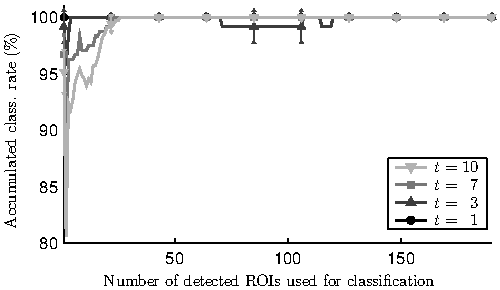
\includegraphics[width=0.46\linewidth]{c2_fig10a} 	
		\label{fig:c2_addVid} }
	\hspace*{4mm}
	\subfloat[Update scenario]{
		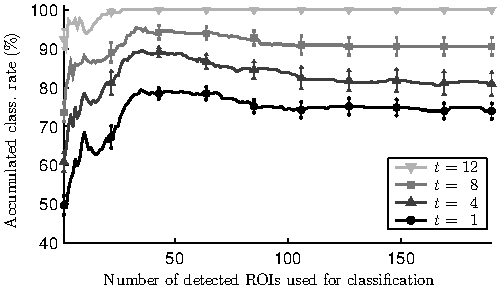
\includegraphics[width=0.46\linewidth]{c2_fig10b} 	
		\label{fig:c2_updVid} }
  }
	\caption{Evolution of the average classification rate for video sequences of the AMCS's ensemble versus the number of ROIs used to identify individuals of the IIT-NRC data base.
Performance is shown for incremental learning under both scenarios for the AMCS with LBESTS$_\text{+d}$.
Error bars correspond to the 90\% confidence interval}
	\label{fig:c2_vid}
\end{figure*}
%--------------- \Classification for video sequences - IIT-NRC ----------------%

As Figure \ref{fig:c2_vid} shows, the video-based classification rate for both scenarios follow the same trends as when the system is tested with single ROIs (Figures \ref{fig:c2_add} and \ref{fig:c2_upd}).
When classes are enrolled incrementally (Figure \ref{fig:c2_addVid}), class decision boundaries becomes more complex in time.
Accuracy obtained with few ROIs then decreases, while the number of ROIs necessary to achieve a video-based classification rate comparable to 100\% increases.
On the other hand, the video-based classification rate obtained after updating classes through incremental learning grows over time, as new blocks of data become available.
When blocks are available, the AMCS needs fewer ROIs to achieve a higher video-based accuracy and it is eventually comparable to 100\% with the same number of ROIs as during enrollment.

The effect on AMCS accuracy of video sequence length used to recognize individuals is also shown in Figure \ref{fig:c2_cmc}.
With each passing ROI, evidence in the form of class predictions is accumulated.
As FAM networks outputs are binary vector, the number of ROIs that predicts a class is instead accumulated and used to establish a ranking through majority voting.
The cumulative match curves in Figure \ref{fig:c2_cmc} show that as the length of the video sequences (and number of ROIs) increases, ambiguity regarding the predictions diminishes.
The probability of the correct class being the first ranked prediction increases to eventually reach 100\%, while the minimal ranking with a cumulative probability of 100\% also decreases to eventually reach 1.

%---------------------------- CMC curves - IIT-NRC ----------------------------%
\begin{figure*}[t]
  \centering
  \fbox{
	\subfloat[Enrollment scenario]{
		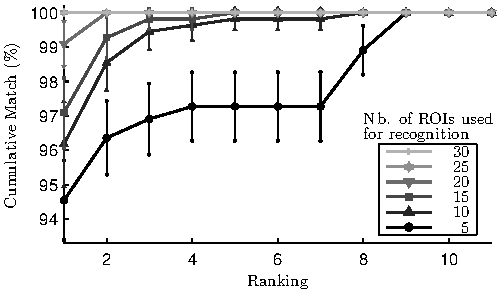
\includegraphics[width=0.46\linewidth]{c2_fig11a} 	
		\label{fig:c2_addcmc} }
	\hspace*{4mm}
	\subfloat[Update scenario]{
		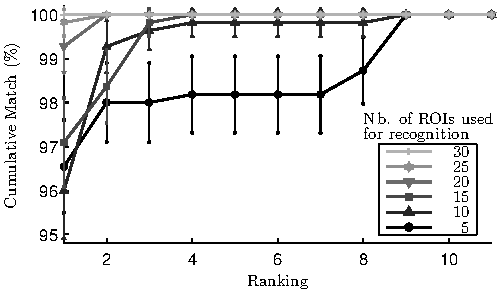
\includegraphics[width=0.46\linewidth]{c2_fig11b} 	
		\label{fig:c2_updcmc} }
  }
	\caption{Cumulative Match Curves the AMCS's ensemble for different number of ROIs used to perform face recognition.
Performance is shown after incremental learning of all the IIT-NRC data base, under both scenarios for the AMCS with LBESTS$_\text{+d}$.
Error bars correspond to the 90\% confidence interval}
	\label{fig:c2_cmc}
\end{figure*}
%--------------------------- \CMC curves - IIT-NRC ----------------------------%

When both learning and test sequences of the IIT-NRC data base were recorded, the individuals were all initially facing the camera, giving a full frontal image of their face.
The ROIs of the first frames are similar leading to classification rates obtained with the first pattern of each video sequences that are always higher than those obtained with a single ROI.
As the individuals begin moving, changing his facial orientation and expression, different facial views, corresponding to data points in new regions of the feature space, are presented to the system.
Since the first frames of each video sequence are initially present in $D_1$, the biometric face models are not well defined and these new regions in the feature space are then unexplored by the FAM networks.
Recognizing an individual toward the end of a video sequence is thus more difficult.
As the number of frames used to perform recognition increases, correct predictions for each ROIs accumulated at the beginning of the test sequences are surpassed by the wrong predictions accumulated with the subsequent ROIs.
Until all classes are updated, this leads to a video-based classification rate that tends to decrease at the end of each sequence. 

%------------------ Number of ROIs necessary to achieve 100% -----------------%
\begin{table*}[t]
	\small
	\centering
	\caption{Number of ROIs necessary to achieve a classification rate comparable to 100\% for video-based face recognition after learning the entire IIT-NRC and MoBo data bases through both incremental learning scenarios with the AMCS}
	\begin{tabular*}{\linewidth}{@{\extracolsep{\fill}}|l||rrr||rr|}
		\hline
		Type of learning &\multicolumn{3}{c||}{Incremental} 
										 &\multicolumn{2}{c|}{Batch} \\ \hline
		Method &\textbf{LBESTS$_\text{+d}$} &SWARM &GBEST &PSO$_\text{B}$ &\textit{k}NN
		\\ \hline
		
		\multicolumn{6}{|l|}{\vspace{-5pt}}\\
		\multicolumn{6}{|l|}{\hspace{-5pt}\textbf{IIT-NRC data base}}			\\\hline
		Number of ROIs during enrollment &24 &23 &never &19 &24 				\\
		Number of ROIs during update     &25 &20 &never &19 &24 				\\\hline
		
		\multicolumn{6}{|l|}{\vspace{-5pt}}\\
		\multicolumn{6}{|l|}{\hspace{-5pt}\textbf{MoBo data base}}				\\\hline
		Number of ROIs during enrollment &15 &30 &16 &32 &16 						\\ 
		Number of ROIs during update     &27 &25 &16 &32 &16 						\\\hline
	\end{tabular*}
	\label{tab:c2_vid}
\end{table*}
%----------------- \Number of ROIs necessary to achieve 100% -----------------%

In the worst case (the update scenario), Table \ref{tab:c2_vid} shows that the AMCS with the DPSO-based strategy needs 5 additional ROIs than with SWARM to have an accuracy comparable to 100\%.
Assuming ideal tracking performances and a camera that acquires video sequences at a rate of 30 frames per second, this represents around a fifth of a second.
This level of performance is also achieved with only a third of the resources (see Table \ref{tab:c2_add} and \ref{tab:c2_upd}). 
The number of additional ROIs needed to achieve a classification rate comparable to 100\% grows to six with ensembles obtained through batch learning of all cumulative data.
Results are similar with the MoBo data base, except for AMCSs with the proposed DPSO-based strategy which require fewer ROIs to achieved a 100\% classification rate.
The more controlled data acquisition conditions for MoBo also make it possible for a single FAM network to achieve a perfect video-based classification rate.

%------------------ Comparison with others - MoBo and IIT-NRC -----------------%
\begin{table*}[t]
% 	\footnotesize
	\small
	\centering
	\caption{Comparison of the DPSO-based learning strategy with other authors on the IIT-NRC and MoBo data bases.
Classification rates where obtained for recognition on video sequences}
	\begin{tabular*}{\linewidth}{@{\extracolsep{\fill}}|l|lllll|}
		\hline
		\multicolumn{6}{|l|}{\vspace{-5pt}}\\
		\multicolumn{6}{|l|}{\textbf{IIT-NRC data base}}
		\\ \hline
		Proposed syst. & Arandjelovic et al. & Gorodnichy &
		Tangelder et al. & Wang et al. & \\
		& (2009) & (2005) & (2006) & (2009) & \\
		100\%  & 100\%  & $95\%$  & $95\%$  & $93\%$ & \\\hline
		
		\multicolumn{6}{|l|}{\vspace{-5pt}}\\
		\multicolumn{6}{|l|}{\hspace{-5pt}\textbf{MoBo data base}}				\\\hline
		Proposed syst. & Cevikalp et al. & Hadid et al. &  Liu et al. &
		Wang et al. & Zhou et al. \\
		& (2010) & (2004) & (2003) & (2008) & (2003) \\
		$100\%$  & $98\%$ & $94\%$  & $99\%$  & $94\%$  & $100\%$
		\\ \hline
	\end{tabular*}
	\label{tab:c2_vsOthers}
\end{table*}
%----------------- \Comparison with others - MoBo and IIT-NRC -----------------%

Compared to other methods proposed in literature for video-based face recognition, an AMCS with the proposed DPSO learning strategy outperforms other systems, except that of \cite{arandjelovic09} with the IIT-NRC data base and \cite{zhou03} with the MoBo data base.
Regardless of the scenario, the AMCS with LBESTS$_\text{+d}$ must accumulate about 1 second of video stream to accumulate the ensemble responses and achieve a classification rates of 100\% after incremental learning of the entire MoBo data base.
In comparison, after performing \emph{batch learning} of the MoBo data base
\cite{zhou03} achieved the same result by accumulating classifier responses for 0.5 second.
While \cite{arandjelovic09} also obtained a 100\% video-based classification rate, the number of accumulated response to achieve this is not available.

%------------------------------------------------------------------------------%
%------------------------------------------------------------------------------%
\subsection{Particle diversity -vs- classifier diversity}
\label{sec:c2_expDiv}

%---------------------------------- Diversity ---------------------------------%
\begin{figure*}[t]
  \centering
  \fbox{
	\subfloat[]{
	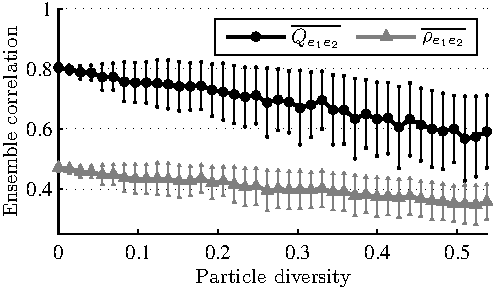
\includegraphics[width=0.46\linewidth]{c2_fig12a} \label{fig:c2_corr} }
	\hspace*{1mm}
	\subfloat[]{
	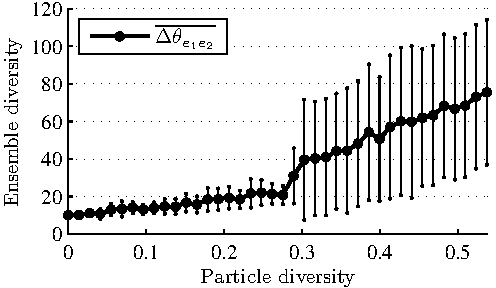
\includegraphics[width=0.46\linewidth]{c2_fig12b} \label{fig:c2_amb} }
  }
  \caption{Ensemble diversity in the classification environment as a function of particle diversity ($\overline{\delta_{e_1e_2}}$) in the optimization environment.
Ensemble diversity is shown using two correlation indicators ($\overline{Q_{e_1e_2}}$ and $\overline{\rho_{e_1e_2}}$ in Figure \ref{fig:c2_corr}), and an diversity indicator ($\overline{\Delta\theta_{e_1e_2}}$ in Figure \ref{fig:c2_amb}).
A decrease in correlation signifies an increase in diversity.
Each indicator is shown with its 90\% confidence interval}
  \label{fig:c2_diversity}
\end{figure*}
%--------------------------------- \Diversity ---------------------------------%

As mentioned, the DPSO-based incremental learning strategy is based on the hypothesis that particle diversity in the hyperparameter space implicitly generates diversity in the feature space, among classifiers associated with those particles.
Based on the experiment introduced in Figure \ref{fig:c2_proof}, this hypothesis is verified.
Figures \ref{fig:c2_diversity} presents the value of three classifiers correlation/diversity indicators -- $Q$ statistic (Equations \ref{eq:c2_Q}), Correlation coefficient (Equation \ref{eq:c2_r}), and the specialized ambiguity indicator for FAM networks (Equation \ref{eq:c2_divFam}) -- as a function of particle diversity in the hyperparameter space (Equation \ref{eq:c2_divPso}) when training on the IIT-NRC data base.
Figures \ref{fig:c2_addDiv} and \ref{fig:c2_updDiv} also show the classifier and particle diversity obtained during incremental learning for AMCS where ensembles are formed with LBESTS$_\text{+d}$ and SWARM.

FAM performs sequential learning of training patterns.
Therefore, decision boundaries created during training depends heavily on patterns presentation order.
Given that this order is typically determined randomly, prior each training epoch, an ensemble's classifiers will differ, even though they were trained with the same hyperparameters (see Figure \ref{fig:c2_diversity}).
When all particles are initially positioned at the global best position, this yields correlation indicators that are lower than one ($\overline{Q_{e_1e_2}}=0.80\pm0.01$ and $\overline{\rho_{e_1e_2}}=0.47\pm0.01$) and a diversity indicator higher than 0 ($\overline{\Delta\theta_{e_1e_2}}=0.07\pm0.01$).

As the hypercube expands (see Figure \ref{fig:c2_proof}), particle swarm diversity increases linearly.
No matter if diversity is computed in the decision space with the correlation indicators based on ensemble disagreement ($\overline{Q_{e_1e_2}}$ and $\overline{\rho_{e_1e_2}}$), or with ambiguity in the feature space ($\overline{\Delta\theta_{e_1e_2}}$), classifier diversity (correlation) follows the same trend by increasing (decreasing) constantly.
Depending on the indicator, diversity in the classification environment changes significantly for different levels of particle diversity: the $Q$ statistic differs for $\overline{\delta_{e_1e_2}}=0.26$ ($\overline{Q_{e_1e_2}}=0.7\pm0.1$), correlation differs for $\overline{\delta_{e_1e_2}}=0.25$ ($\overline{\rho_{e_1e_2}}=0.41\pm0.06$), and ambiguity-based diversity differs for $\overline{\delta_{e_1e_2}}=0.09$ ($\overline{\Delta\tau_{e_1e_2}}=0.10\pm0.02$).
Overall, results confirm the initial hypothesis that diversity in the hyperparameter space does indeed translates to diversity among classifiers in the feature space.

It is important to note that FAM networks are very sensitive to the match tracking hyperparameter ($\epsilon$) when it is close to zero.
Indeed, positive and negative values of $\epsilon$ have opposite effect on the dept of search performed among $F_2$ nodes when training on a pattern $\textbf{a}$.
When a winning $F_2$ node $j^*$ leads to a prediction error, positive (negative) values of $\epsilon$ restricts (relaxes) the condition on which subsequent $F_2$ nodes passes the vigilance test.
With $\epsilon>0$ ($\epsilon<0$), FAM tends to create more (fewer), but smaller (larger), category hyper-rectangles, leading to narrow (broad) generalization.
This explains the large confidence interval observed when $\overline{\delta_{e_1e_2}} > 0.3$.
For two out of ten replications, the global best position found during DPSO optimization leads to global optimal values with $\epsilon \in [-0.03, 0.06]$. 
When particle diversity reaches $\delta=0.3$, ensembles are then formed of classifiers with both positive and negative match tracking values, leading to a considerable classifier diversity ($\overline{\Delta\theta_{e_1e_2}} > 200$).

%------------------- Particles - Diversity during enrollment ------------------%
\begin{figure*}[t]
  \centering
  \fbox{\begin{minipage}{0.97\linewidth}\centering
	%-- Diversity
	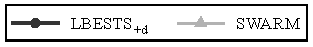
\includegraphics[width=0.4\linewidth]{c2_fig13-14_leg} \\
	\subfloat[Particle diversity]{
		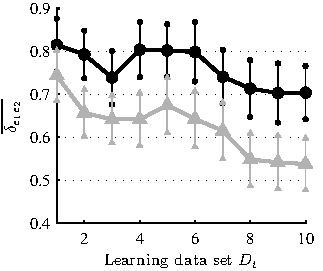
\includegraphics[width=0.31\linewidth]{c2_fig13a} 
		\label{fig:c2_addDivSwm} }
	\hspace*{1.5mm}
	\subfloat[Classifier diversity]{
		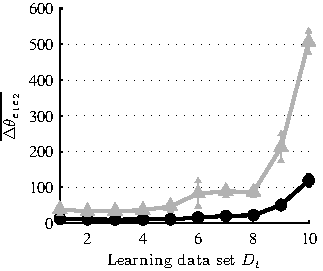
\includegraphics[width=0.31\linewidth]{c2_fig13b} 	
		\label{fig:c2_addDivFam} }
	\hspace*{1.5mm}
	\subfloat[Scatter plot]{
		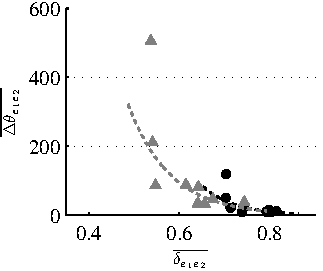
\includegraphics[width=0.31\linewidth]{c2_fig13c} 	
		\label{fig:c2_addDivCor} }
  \end{minipage} }
	\caption{Particle and classifier diversity of the AMCS's ensembles versus the number of learning blocks during the enrollment learning scenario (Figures \ref{fig:c2_addDivSwm} and \ref{fig:c2_addDivFam}).
The FAM ambiguity indicator (Equation \ref{eq:c2_divFam}) was used for classifier diversity and all results are presented with their 90\% confidence interval.
Also shown is classifier diversity as a function of the particle diversity using all data points (Figure \ref{fig:c2_addDivCor})}
	\label{fig:c2_addDiv}
\end{figure*}
%------------------ /Particles - Diversity during enrollment ------------------%

%--------------------- Particles - diversity during update --------------------%
\begin{figure*}[t]
  \centering
  \fbox{\begin{minipage}{0.97\linewidth}\centering
	%-- Diversity
	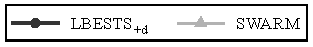
\includegraphics[width=0.4\linewidth]{c2_fig13-14_leg} \\
	\subfloat[Particle diversity]{
		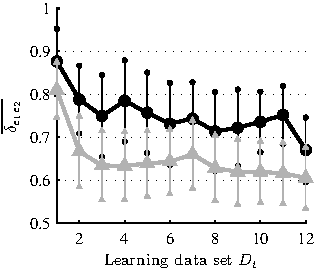
\includegraphics[width=0.31\linewidth]{c2_fig14a} 	
		\label{fig:c2_updDivSwm} }
	\hspace*{1.5mm}
	\subfloat[Classifier diversity]{
		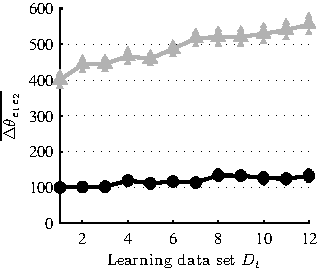
\includegraphics[width=0.31\linewidth]{c2_fig14b} 	
		\label{fig:c2_updDivFam} }
	\hspace*{1.5mm}
	\subfloat[Scatter plot]{
		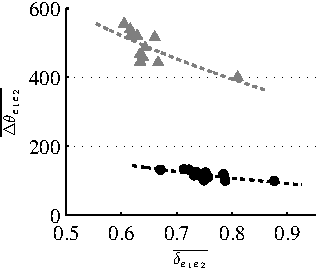
\includegraphics[width=0.31\linewidth]{c2_fig14c} 	
		\label{fig:c2_updDivCor} }
  \end{minipage} }
	\caption{Particle and classifier diversity of the AMCS's ensemble versus the number of learning block during the update learning scenario (Figures \ref{fig:c2_updDivSwm} and \ref{fig:c2_updDivFam}).
The ambiguity indicator (Equation \ref{eq:c2_divFam}) was used for classifier diversity and all results are presented with their 90\% confidence interval.
Also shown is the classifier diversity as a function of the particle diversity using all data points (Figure \ref{fig:c2_updDivCor})}
	\label{fig:c2_updDiv}
\end{figure*}
%-------------------- /Particles - diversity during update --------------------%

However, as results shown in Figures \ref{fig:c2_addDiv} and \ref{fig:c2_updDiv}, the relation between particle and classifier diversity during incremental learning is not as simple as with batch learning.
When data is learned incrementally over time, FAM decisions boundaries may be adjusted to accommodate new classes.
In the hyperparameter space, the objective function changes over time and regions with potential optima become increasingly localized (\cite{connolly10}).
Diversity in the hyperparameter space then decreases gradually, and convergence of subswarms toward local optima reduces particle swarm diversity below that obtained with the greedy search process. 
Under the update scenario, all classes are represented at the beginning of the learning process, and FAM networks are more complex, which increases the impact of the hyperparameters used during training.
Even if particle diversity values for $D_1$ are lower than those obtained during enrollment, classifier diversity is typically about ten times higher.
This increased complexity leads to an increased variation across the different replications, resulting in larger confidence intervals for particle diversity.
Even if results are comparable for AMCSs with LBESTS$_\text{+d}$ and SWARM (Figure \ref{fig:c2_updDivSwm}), LBESTS$_\text{+d}$ still tends to provide the highest particle diversity.

Meanwhile, in the feature space, FAM networks are trained using different hyperparameters and different pattern presentation orders with each passing $D_t$.
As shown in Figure \ref{fig:c2_addDiv}, as new data is learned by the AMCS, the ensemble of classifiers becomes increasingly diverse.
Figures \ref{fig:c2_addDivCor} and \ref{fig:c2_updDivCor} illustrate that, in a context of incremental learning, there is an inverse relationship between particle and classifier diversity.
As mentioned, the higher ensemble diversity observed with SWARM does not translate to a significantly higher classification rate for the ensemble.

Note that this does not contradict results presented in Figure \ref{fig:c2_diversity}, where a diversity analysis is performed with FAM networks that are initially all in the same state prior learning the whole IIT-NRC data base with batch learning.
Instead, for each learning data set $D_t$, Figures \ref{fig:c2_addDiv} and \ref{fig:c2_updDiv} present only one point in the particle--classifier diversity space of what is a diversity analysis when using the greedy search process (Algorithm \ref{alg:c2_ens}) on a local time frame and with networks that are in different initial conditions.

%--------------------------------- Conclusion ---------------------------------%
\section{Conclusion} \label{sec:c2_conclusion}

%-- Paper objective
In this chapter, an incremental learning strategy based on DPSO is proposed to evolve heterogeneous ensembles of classifiers in response to new data.
This strategy is applied to an AMCS for video-based face recognition consisting of a pool of FAM neural networks to classify face regions, the DNPSO algorithm to optimize classifier parameters such that classification rate is maximized.
The dynamic swarm properties are then exploited to perform an ensemble selection process based on accuracy and diversity.

Overall results confirm that there is indeed a correlation between diversity in the optimization environment and diversity in the classification environment.
The diversity of solutions can easily be controlled in the optimization environment with a DPSO algorithm, and allows for an efficient selection of diversified ensembles of classifiers.
When the AMCS uses the DPSO learning strategy, the best results are thus obtained by combining the neural networks associated to the local best particles with a greedy search that aims to maximize particle diversity in the hyperparameter space.
Although this approach does not ensure finding an ensemble with the global optimum particle diversity, this search algorithm allows to select ensembles that yield classification rates comparable to that of reference ensemble-based and batch learning techniques, but with only a fraction of the resources and without the need to assess diversity among classifiers in the feature or decision space.

%While the classifiers evolved using the DPSO-based learning strategy are defined according to the personal best position of each particle, the mechanisms for DPSO subswarms creation proposed in the literature adjust instead the current position of the swarm.
%Moreover, as with most DPSO algorithms, DNPSO focuses on detecting and tracking the objective function's local optima.
%Even if this allows optimization in a dynamic environment, evolving a swarm of neural networks also requires maintaining diversity around each local optima to maximize the effect of the greedy search.
%Future work should involve devising a DPSO algorithm that circumvent those issues  and is specifically aimed at the creation of diversified pool of classifiers within the AMCS framework.
%A majority vote is employed for classifier fusion, although further studies should be made to determine an optimal fusion function according to ensembles selected through the DPSO-based strategy.
%Moreover, one could define criteria to specify the face samples from each learning block $D_t$ that are selected for the long term memory (LTM) to provide the highest performance. 
%Validation and fitness estimation (respectively done during the learning and optimization processes) would therefore be performed using the most representative data of each class distribution.